\documentclass[12pt]{article}

%package to include pdf
\usepackage{pdfpages}

% For code listing
\usepackage{listings}
\usepackage{color}

% Another code listing package
\usepackage{minted}

% For links and hyperreferences
\usepackage{hyperref}
\hypersetup{
    colorlinks=true,
    linkcolor=blue,
    filecolor=magenta,      
    urlcolor=cyan,
}

\usepackage{subcaption}

% Package to display directory tree
\usepackage{forest}

\definecolor{folderbg}{RGB}{124,166,198}
\definecolor{folderborder}{RGB}{110,144,169}

\def\Size{4pt}
\tikzset{
      folder/.pic={
        \filldraw[draw=folderborder,top color=folderbg!50,bottom color=folderbg]
          (-1.05*\Size,0.2\Size+5pt) rectangle ++(.75*\Size,-0.2\Size-5pt);  
        \filldraw[draw=folderborder,top color=folderbg!50,bottom color=folderbg]
          (-1.15*\Size,-\Size) rectangle (1.15*\Size,\Size);
      }
    }


% Wrapping text around figures (doesn't work)
\usepackage{wrapfig}
% Figures with side caption
\usepackage[rightcaption]{sidecap}
% Fancy header and footer package
\usepackage{fancyhdr}
\pagestyle{fancy}
\fancyhf{}
\fancyhead[R]{UON parser}
\fancyhead[L]{\rightmark}
%\fancyfoot[L]{\leftmark}
\fancyfoot[R]{\thepage}

\renewcommand{\headrulewidth}{0.5pt}
\renewcommand{\footrulewidth}{0.5pt}

\definecolor{mygreen}{rgb}{0,0.6,0}
\definecolor{mygray}{rgb}{0.5,0.5,0.5}
\definecolor{mymauve}{rgb}{0.58,0,0.82}

\lstset{ %
  backgroundcolor=\color{white},   % choose the background color
  basicstyle=\footnotesize,        % size of fonts used for the code
  breaklines=true,                 % automatic line breaking only at whitespace
  captionpos=b,                    % sets the caption-position to bottom
  commentstyle=\color{mygreen},    % comment style
  escapeinside={\%*}{*)},          % if you want to add LaTeX within your code
  keywordstyle=\color{blue},       % keyword style
  stringstyle=\color{mymauve},     % string literal style
}

% Set up data, if you need to add a package, go here
\input{setup/packages.tex}

\begin{document}


\thispagestyle{empty}
\setlength\headheight{0pt} 
\begin{center}

\begin{center}
\includegraphics[width=0.70\linewidth]{images/HEIG-VD_Logo.eps}            
\end{center}	

        %\vspace{0.25cm}
        %{\scshape\LARGE TU Dublin, Tallaght Campus \par}
        %\vspace{0.25cm}
        %{\scshape\Large BSc / HDip / MSc Project Template\par}
        %\vspace{0.5cm}
        \vspace*{\fill}
        {\Large\bfseries Parser for a serialization language UON™\par}
        
        \vspace{0.5cm}
        {\Large\itshape Stephane Selim\par}
        Department of TIC \\
        Orientation IL
        \vspace{0.25cm}

\vspace{1cm}
Subject proposed by\par
Prof. Yves Chevallier \\
Department of TIN\par

\vspace{1cm}
Supervised by\par
Prof. Yves Chevallier \\
Department of TIN\par

\vspace{1cm}
Academic Year\par
2019-2020\par

\large
\vfill
\begin{flushright}
Yverdon-les-Bains, \today
\end{flushright}

\vspace*{\fill}
\end{center}

\clearpage
\restoregeometry
\justify

\vspace*{\fill}
\begin{center}
\section{Foreword}  
This Bachelor project (hereinafter TB for "Travail de Bachelor") is carried out at the end of the school curriculum, in preparation for obtaining the title of Bachelor of Science HES-SO in Engineering.

As an academic work, its content, without prejudging its value, engages neither the responsibility of the author, nor that of the jury of the Bachelor project and the School.

Any use, even partial, of this TB must be made in accordance with copyright.

\vfill
\begin{flushright}
HEIG-VD

Dean name: Vincent Peiris \break
Head of TIC Department
\end{flushright}

\vfill
\begin{flushleft}
Yverdon-les-Bains, \today
\end{flushleft}

\end{center}
\vspace*{\fill}

\pagebreak

\vspace*{\fill}
\begin{center}
\section{Declaration}

I, the undersigned Stephane Selim, hereby certifies having carried out this work alone and having not used any other source than those expressly mentioned.

\vfill
\begin{flushleft}
Yverdon-les-Bains, \today
\end{flushleft}

\vfill
\begin{flushright}
Stephane Selim
\end{flushright}

\end{center}
\vspace*{\fill}

\pagebreak

\section{Prcoject specifications (Cahier des Charges)}
\begin{enumerate}
    \item Exploring parser techonologies in Python.
    \item Write a functional UON grammar.
    \item Parse UON into a set of Python objects.
    \item Coercion between UON types.
    \item Binary encoding and decoding of UON objects.
    \item Schema and data validation.
\end{enumerate}

Here is a broad outline of the project timeline. First, it is decided that this project will be implemented in Python, so the first step is to explore existing parser technologies and libraries in Python.

After a parser technology has been chosen, we have to write the smallest functioning subset of a UON grammar as a starting point, and then build on it. We will then proceed to transforming the parsed UON into corresponding Python objects. These Python objects should represent the different native data types supported by UON. 

A UON class hierarchy should be established, along with their methods and attributes to have a full set of Python objects, that we're able to parse UON into.

Once the grammar and the Python objects are fixed, we will experiment with type coercion between the different UON Python objects. For example if a floating point number was to be coerced in UON to an integer, the resulting Python object should reflect that type coercion.

We will implement binary encoding and decoding of the different UON types. Every UON type has its own binary encoding according the specification and the decoding should follow the same pattern.

Finally, we will have to implement a basic Schema validation based on those Python objects.

\pagebreak

\tableofcontents
\pagebreak

\section{Introduction}
The following Bachelor project consists of implementing a parser for the newly created serialization language UON (which stands for Unified Object Notation). In the following, we will present the motivation behind this new serialization language, the specification for this language and how we went about implementing a parser for it. In detail, we will see the incentive behind designing a new serialization language in an already crowded field, we will see what makes it stand out among the others well known like JSON, XML or YAML and how it accomplishes specific needs compared to the others. We will present the key aspects of the specification of the language. We will then present the implementation, the tools and the choices we’ve taken at every stage of the parser, starting with the grammar of the language to the processing of the final resulting AST (Abstract Syntax Tree).

\pagebreak

\section{Pre-Study}
UON is a newcomer to the field of data serialization. To understand how UON stands out among its already established peers like JSON or YAML, we need to delve into the world of serialization and have a look at what serialization does and what UON offers that others don’t.

\subsection{Serialization}
We live in a heterogeneous world where data is constantly moved and transferred from one endpoint to another. But the way these endpoints interpret the data and store it is not the same from one another. So we need some way to send the data that is platform and language-agnostic. We need to \textbf{serialize} the data, that is transform it into a format that can be understood by all platforms. This is the main reason we serialize data for.

For example, say we have a Java class Person with attributes name and age. A Java object of this class would be as follows:

\begin{lstlisting}[language=java]
Person person = new Person("Fred", 28);
\end{lstlisting}

Now you need to send that data over to another endpoint that only runs on Python. How would you go about sending that data onto the network and how do you expect Python to interpret it? Python only understands Python classes and you’re sending him a Java Object.
Here is when serialization comes in handy. You make the Java class Person \emph{Serializable} (by implementing its interface) and you translate the object into some serialization format such as the well-known JSON:

\begin{lstlisting}{language=json}
{
  Person: {
    "name": "Fred",
    "age": 28 
  }
}
\end{lstlisting}

\hfill\break
Or XML: 

\begin{lstlisting}[language=xml]
<Person>
  <name> Fred </name>
  <age> 28 </age>
</Person>
\end{lstlisting}

and you send it over the network. When Python receives the data, he \emph{deserialize}s it to rebuild the original data, now as a Python object of type Person of which you already created a Python class for it.

\subsubsection{Definition}
More formally, from the definition taken from the microsoft Docs, \textbf{serialization} can be defined as the process of storing the state of an object to a storage medium. During this process, the public and private fields of the object and the name of the class, including the assembly containing the class, are converted to a stream of bytes, which is then written to a data stream. When the object is subsequently deserialized, an exact clone of the original object is created. It can be used as we said when we want to transfer data over a network, or when we want to store data on a medium such as hard disks or databases or any other situation where you’d want to store data in a format that is independent of the architecture or the platform.

\begin{figure}[ht!]
 	\centering
 	\caption{Serialization process}
 	\includegraphics[width=0.7\linewidth]{images/Serialization/serialization_illustration.eps}
 	\label{lab:perceptron}
\end{figure}

So when we said that Java objects can be serialized as in the previous example, we weren’t entirely accurate. In the previous example, we converted the object to a JSON object, which of course you can, but Java also has its own internal serialization process. The java object to be serialized must implement the interface \emph{java.io.Serializable} (or its subinterface \emph{java.io.Externalizable} if you want more control of how serialization is done on your object), this flags the class as valid for serialization. Then you can use an \emph{OutputStream} to write the data of the object of this class to a file or to a socket. The output will be a byte stream so you can’t really read it with your eyes but it will contain all the data of the object, as well information on the class itself. So it can now be effectively read by another computer or another program and correctly reconstruct the data.

Here is another example that I find very illustrative:

\begin{figure}[ht!]
 	\centering
 	\caption{Serialization process}
 	\includegraphics[width=3cm, height=8cm]{images/Serialization/serialization_image_example.png}
 	\label{lab:perceptron}
\end{figure}

When you send an image over the internet, the same process happens. The image and its data are serialized. Just as the way you store an image in SQL database, you save it in a Blob, which is essentially converting the image into a stream of bytes (hence the name Binary large object).


% \begin{wrapfigure}{r}{0.5\textwidth}
%   \begin{center}
%     \includegraphics[width=0.48\textwidth]{images/Serialization/serialization.png}
%   \end{center}
%   \caption{Birds}
% \end{wrapfigure}

\subsection{Serialization formats}
When you serialize the data, we’ve seen that you can serialize in either binary format or in a text format. So the question you would want to ask yourself is why choose one over the other and what advantages does this have?

Text format is human-readable, which is in itself a big plus. In contrast, binary format is generally faster to process, which is endemic to binary encoding itself. Binary content is more compact than its text counterpart since the latter required more bytes. Thus we find ourselves with increased performance and efficiency of access when working with binary.

\subsection{Benchmarks}\label{benchmarks}
To test the difference in performance between binary and text format serialization, we’ve run a small benchmark test done in Python, between binary formats like BSON and Msgpack, and text formats like JSON and YAML, on the following data :

\begin{lstlisting}[language=python]
data = {
   "name": "Jack",
   "age" : 28,
   "hobbies" : ["skating", "eating", "jogging"],
   "description": """Lorem ipsum dolor sit amet, consectetur adipiscing elit, sed do eiusmod tempor incididunt ut
               labore et dolore magna aliqua. Ut enim ad minim veniam, quis nostrud exercitation ullamco laboris nisi
               ut aliquip ex ea commodo consequat. Duis aute irure dolor in reprehenderit in voluptate velit esse cillum
               dolore eu fugiat nulla pariatur. Excepteur sint occaecat cupidatat non proident, sunt in culpa qui officia
               deserunt mollit anim id est laborum. """
}
\end{lstlisting}

 We’ve used the official Python libraries for each of these formats to run these tests. Here are the results (measured in seconds as a float) of 10000 iterations for each test:
 \hfill\break

\subsubsection{BSON}
\begin{lstlisting}[language=python]
 s = '''
 a = bson.dumps(data)
 b = bson.loads(a)
 '''
 print("BSON time: ", timeit.timeit(setup=mysetup, stmt= s, number=10000))
\end{lstlisting}

Using \href{https://github.com/py-bson/bson}{bson from py-bson}
We get BSON time:  0.91669s.

\subsubsection{JSON}
\begin{lstlisting}[language=python]
  s_json = '''
 a = json.dumps(data)
 b = json.loads(a)
 '''
 print("JSON time: ", timeit.timeit(setup=mysetup_json, stmt= s_json, number=10000))
\end{lstlisting}

Using the in-built module \href{https://docs.python.org/3/library/json.html}{json}
We get JSON time:  0.20858s.

\subsubsection{Msgpack}
\begin{lstlisting}[language=python]
 s_msgpack = '''
 a = msgpack.packb(data, use_bin_type=True)
 b = msgpack.unpackb(a, raw=False)
 '''
 print("MsgPack time: ", timeit.timeit(setup=mysetup_msgpack, stmt= s_msgpack, number=10000))

\end{lstlisting}

Using the \href{https://github.com/msgpack/msgpack-python}{msgpack module}
We get MsgPack time:  0.070190s.

\subsubsection{YAML}
\begin{lstlisting}[language=python]
 s_yaml = '''
 a = yaml.dump(data)
 b = yaml.load(a, Loader=yaml.FullLoader)
 '''
 print("YAML time: ", timeit.timeit(setup=mysetup_yaml, stmt= s_yaml, number=10000))

\end{lstlisting}

Using the \href{https://pyyaml.org/wiki/PyYAMLDocumentation}{PyYAML module}
We get a whopping YAML time:  41.1645s!

We see that MsgPack has the fastest time compared to the second best JSON, with a factor of 2 or 3 times as fast, which is due to the binary serialization of msgPack. By contrast YAML, which is the most human readable of them all,  has the slowest recorded performance with a factor of at least 200x slower than JSON’s! This is due to the inherent complexity of the YAML specification which translates into its parsers as well.

One small inconsistency that we noticed is BSON’s performance. BSON is binary serialization and while it’s still fast, it records performance time slower than that of JSON’s. Why? Well this is probably not due to the format itself but to the environment in which it is executed. We’ve run these tests in Python but this problem was also present in Node.js \href{https://stackoverflow.com/questions/36767310/why-is-json-faster-than-bson-in-node-js}{[2]}. In most environments, binary encodings would be easier to encode but some formats like JSON have in-built serialization in the environment that is implemented in native code and in an optimised fashion. This might be what is happening in Python as well. The in-built \emph{json} module might be more optimised than bson’s python module (which is actually an Independent BSON codec for Python that doesn’t depend on MongoDB’s BSON). This explains the difference in performance between the two formats in this particular case.

As a rule of thumb, if you’re looking for a format that is heavy on performance and requires less storage space, binary serialization might be what you’re looking for. Otherwise you’re better off with text based format, especially when you’re constantly checking your data, for example during debugging, and you don’t want to go through other tools to be able to read your data.

\pagebreak

\subsection{Overview of some serialization formats}

\subsubsection{JSON}
JSON (JavaScript Object Notation) is a lightweight data-interchange text-format that is based on a subset of the JavaScript Programming Language. Since JavaScript is used across the web, this makes JSON the de facto leader of serialization formats when it comes to web applications. \href{https://www.json.org/json-en.html}{[3]}

It has dominated the field with its minimal and human-readable format. It has become an alternative to the well-established XML as a way of transmitting data between servers and web applications. Developers love it for its simplicity and its structuring of data.

It is built on two structures:
\begin{itemize}
    \item A collection of key/value pairs. This represents an equivalent data structure in most programming languages like Maps in Java or dictionaries in Python.
    \item An ordered list of values. This also represents an equivalent data structure in most programming languages like lists, sequences or arrays (which represent the same thing: an ordered set of values, with each having its own index in the structure).
\end{itemize}

The representation of these structures mimic those of Python. Given these two simple structures, the format has a very simple syntax grammar and most programming languages are equipped with parsers for this format. The simplicity of this format has allowed some of the parsers to be very well optimized, like JavaScript which is natively optimized for dealing with JSON. 

Example:
\begin{minted}{json}
{
  "firstName": "John",
  "lastName": "Smith",
  "age": 27,
  "address": {
    "streetAddress": "21 2nd Street",
    "city": "New York",
  } ,
 "children": [],
  "hobbies": ["Jogging", "Reading"]
}
\end{minted}

Notes: Data structures can be nested. Strings need to be delimited with double-quotes and support backslash escaping syntax. It doesn’t support comments however.

\subsubsection{YAML}
Yaml, short for Yet Another Markup Language originally, and then retconned later to be a recursive acronym for YAML Ain't Markup Language,  referring more accurately to its purpose of data serialization rather than a mere document markup format. 
YAML has taken the step forward to be more human-readable than JSON. It’s so human-readable that they made the home page of YAML in YAML \href{https://yaml.org/}{[4]}. But this comes at a cost of a much, much bigger specification and grammar complexity. They have already gone through three specifications. They are currently at YAML 1.2, which added compliance with JSON as an official subset. That means that as of YAML 1.2, JSON will be recognized as valid YAML.

It features 3 primitives: mapping (hashes/dictionaries), sequences (arrays, lists) and scalars (strings/numbers). YAML leverages these primitives, and adds a simple typing system and aliasing mechanism to form a complete language for serialization of any native data structure. While most programming languages can use YAML for data serialization, YAML excels in working with those languages that are fundamentally built around the three basic primitives. It also uses whitespace indentation (like Python) to indicate nesting so there is no need for quotes or brackets which makes it more compact.

Owing to its readability and its compact form, it has become widely used, for example for writing configuration files, with tools such as Ansible or Docker adopting the format to write their configuration files.

It also comes with a wide range of parsers in many languages, each one more complicated as the other, to keep up with the format complexity and its defined types. Creating a fully compliant parser with YAML has proven almost impossible \href{https://github.com/yaml/yaml-grammar}{[5]}. This will almost certainly be reflected in the implementation of a parser for UON, the format of which very closely resembles YAML.

Here is an example:

\begin{lstlisting}
- name: John Smith
  age : 27
  address:
     streetAddress :  21 2nd Street
     city: New York
  hobbies: [Jogging, Reading]
- {name : Maggie Smith,
   age : 28}
\end{lstlisting}

\subsubsection{XML}
XML (eXtensible Markup Language) appeared in the mid-1990s as a successor to SGML ( Standard Generalized Markup Language).  Best known for its use in the web early on. It is strictly text-format, but a binary XML version has been proposed to have a more compact format.\href{https://www.w3.org/2003/08/binary-interchange-workshop/29-MicrosoftPosition.htm}{[6]}

XML is a markup format based on tags. Each XML document contains one or more elements, the boundaries of which are either defined by <start-tags>, <end-tags> or empty-element tag for empty elements. Each starting tag must be closed by a closing tag and tags can contain attributes. Elements can contain other elements. This gives a logical structure to the document.
XML can also be validated using a schema like DTD (document type definition) that defines grammatical rules that the XML document must follow. 

Here is an example:
\begin{minted}{xml}
<People>
   <Person>
      <name>John Smith</name>
      <age>2</age>
      <address category="nested">
         <street>21 2nd Street</street>
         <city>New York</city>
      </address>
   </Person>
   <Person>
      <name>Maggie Smith</name>
      <age>28</age>
   </Person>
</People>
\end{minted}

The format is well-formed but, as you may have noticed, it is very verbose and redundant, which is a well-known downside of XML with restrictions such as opening tags must be closed. It is still a text human-readable format but less so compared to others. You can easily get lost between the tags when reading an XML document. The added level of sophistication of this format can also be seen in its parsers, when trying to translate it into code objects. Speaking from personal experience, it can get quite tricky especially with XML elements that come with attributes.

We see it slowly being replaced by the much more concise and simple JSON, since developers will almost always value simplicity over anything else. 

\subsubsection{BSON}
BSON (“Binary JSON”) is a binary serialization format \href{http://bsonspec.org/spec.html}{[7]}. It has been developed internally by MongoDB \href{https://www.mongodb.com/json-and-bson}{[8]} and Mongo uses it as a data storage and network transfer format for its database. But it can also be used outside MongoDB.

It is basically the binary encoding of JSON-like documents (which are UTF-8 String encoded). So it still keeps the ordered key/values pairs structure, but everything is binary. Apart from encoding, it also keeps the length information of the document to make the document traversal when parsing it faster. It supports numeric types that are not native to JSON, representing different precisions such as int32, int64, uint64, double or decimal128. This is convenient when parsing in a language that supports these different sized integers.  It also adds more native types like the “BinData” data type to represent an array of bytes.  

Here are examples taken from the MongoDB’s “JSON and BSON” page when serializing some basic data structures from languages like JavaScript and Python :

\begin{figure}[ht!]
 	\centering
 	\caption{Binary Serialization with BSON 1}
 	\includegraphics[width=0.7\linewidth]{images/Serialization/BSON_example_1.png}
 	\label{lab:perceptron}
\end{figure}

\begin{figure}[ht!]
 	\centering
 	\caption{Binary Serialization with BSON 2}
 	\includegraphics[width=0.7\linewidth]{images/Serialization/BSON_example_2.png}
 	\label{lab:perceptron}
\end{figure}

\subsubsection{Protocol Buffers}
Another example of the well-known binary serialization formats are Google’s Protocol buffers, Protocol buffers are a language-neutral, platform-neutral, extensible mechanism for serializing structured data \href{https://developers.google.com/protocol-buffers}{[9]}. There’s not a better way to explain what PBs are except to cite Google’s Protocol Buffers page itself: “Protocol buffers are a flexible, efficient, automated mechanism for serializing structured data – think XML, but smaller, faster, and simpler. You define how you want your data to be structured once, then you can use special generated source code to easily write and read your structured data to and from a variety of data streams and using a variety of languages. You can even update your data structure without breaking deployed programs that are compiled against the "old" format.”

First you specify how you want your serialized data to be structured in \emph{.proto} files which have a specific format you have to respect. Here is an example of one such file: 

\begin{lstlisting}
message Person {
  required string name = 1;
  optional string nickname = 2;
  required int32 age = 3;

  message Address {
    required string street = 1;
    optional string number = 2;
  }
}
\end{lstlisting}

message Person {
  required string name = 1;
  optional string nickname = 2;
  required int32 age = 3;

  message Address {
    required string street = 1;
    optional string number = 2;
  }
}

Each protocol buffer message is a small logical record of information containing a series of uniquely numbered fields, one for each piece of data you want to include in that type of message. Each field has a name and a value type. The unique number of the fields is used to identify them in the message binary format. You can specify \emph{required} fields, \emph{optional} fields and \emph{repeated} fields. You can nest messages inside others to have a hierarchical structure. The scalar fields like the ones in the example above are of type string or int32. But Protocol Buffers also supports a multitude of data types with different precisions such as int64, uint32, uint64, double, float and so on \href{https://developers.google.com/protocol-buffers/docs/proto#scalar}{[10]}. When a message is encoded, the keys and values are concatenated into a byte stream. On the receiving-end of a protocol buffer message, the decoding apparatus references the \emph{.proto} file to reconstruct the original message. 

Since it’s binary, protocol buffer serialization is fast. As Google draws the comparison with XML, it is 3 to 10 times smaller, 20 to 100 times faster and less ambiguous than XML. It can also generate data access classes that are easier to use programmatically which is very convenient for the developer that wants to work with this data when he receives it. For instance with the example above, compiling the \emph{.proto} file would generate a Person class with attributes for name, nickname and age and would define getters and setters for it.

\subsection{Performance comparison}

The following is the result of some of the benchmark tests done by other people that I found on the internet, to compare the speed and size performance of a selection of serialization formats. These were not performed by me on my local computer so there is no way to verify them and should always be taken with a grain of salt. However the results correspond more or less to the actual performances of these serialization formats and the conclusions drawn by me. Please refer to subsection \ref{benchmarks} for the benchmark tests that were run by me on my local computer, on Python.

The following tests were done in \href{https://blog.mbedded.ninja/programming/serialization-formats/a-comparison-of-serialization-formats/#speed-comparison-benchmarking}{this 2019 blog}, so they are still fairly new at the time of writing this report. It compares the speed and file size between JSON, XML, protocol buffers, TOML, YAML and CSV (which is still considered a serialization format used to represent data). The serialization/deserialization is done using libraries for each of these formats in Python and C++. The sample data to be serialized consists of a \emph{vector} in C++ or a \emph{list} in Python of a \emph{Person} data structure (or class in Python).

\begin{figure}[h]

\begin{subfigure}{0.4\textwidth}
\includegraphics[width=0.9\linewidth, height=5cm]{images/Performance Comparison/mbedded_ninja_performance_c.png} 
\caption{C++ performance comparison}
\label{fig:subim1}
\end{subfigure}
\hfill
\begin{subfigure}{0.4\textwidth}
\includegraphics[width=0.9\linewidth, height=5cm]{images/Performance Comparison/mbeded_ninja_performance_python.png}
\caption{Python performance comparison}
\label{fig:subim2}
\end{subfigure}
\caption{Serialization and deserialization comparison}
\label{fig:image2}
\end{figure}

As we’ve seen the speed comparison results correspond more or less to those that we’ve got above in subsection \ref{benchmarks}. YAML, as to its complexity, takes a huge amount of time compared to others.  And after comes TOML which is also a YAML-like serialization format that aims to be very human-readable at the cost of complexity of its structure. Protocol buffers as expected have very good performance in both programming languages. Now the results of these tests have been taken from the minimum of several runs, and the results can also vary depending on the library used for a serialization format. A performance degradation from one programming language to another may be inherent to the language (C code being a lot faster than Python) or just a case of a badly written serialization library. 
But this gives a general idea of the performance of different serialization formats, and how the complexity of a serialization format is reflected into its performance.

This was only an overview of some of the serialization formats that are available today. We went over the most used and which ones people are most likely to use in their serialization needs and applications, but there are a lot more out there that suit different needs. For a more comprehensive view over the ensemble of the formats, Wikipedia provides a very good and exhaustive comparison between a lot of serialization formats, on certain points and features like binary support or human-readability. \href{https://en.wikipedia.org/wiki/Comparison_of_data-serialization_formats}{[11]}

\pagebreak

\subsection{UON}
We’ve seen the most used serialization formats, what really defines them and makes them stand out amongst others, as well as some of their shortcomings. UON (short for Unified Object Notation) is a new proposed serialization format that seeks to regroup the best features of these serialization formats into one format that encompasses them all. 

\subsubsection{Why UON?}
The main motivation behind UON is to serve the needs of \href{https://en.wikipedia.org/wiki/Industry_4.0}{Industry 4.0}, the 4th revolution that has occurred in the industry. It is not just a buzzword, it is actually happening all around us where traditional practises of the industry are replaced by the latest smart technology within the large scale m2m (machine to machine) communication and Internet of Things (IoT) deployments. This increased automation is shown in the huge amount of computers that are connected and communicate with one another to make decisions without human intervention. This process incurs a huge amount of information and data that are circulated around and the machines involved usually have very limited computation power (we’re not talking about full-blown pc with an ssd and ram, we’re talking about small devices like sensors and controllers and such). 

This begs for some serialization format that could be convenient for encapsulating and representing that data, in the smallest payload possible.
UON hopes to fill this need. Other serialization formats may fulfill specific needs:  JSON with its simplicity satisfies the Web APIs developers, protocol buffers with its concise binary format, interoperability and schema validation, but UON aims to be ubiquitous covering a wide range of applications from battery-powered telemetry sensors to Web communication protocols. For that UON defines a way to :

\begin{itemize}
  \item encode/decode payloads written in binary or in human-readable form
  \item Describe a payload through a validation schema
\end{itemize}

\subsubsection{What is UON?}
UON is a data serialization format. It is meant to be UTF-8 encoded by default, but compatible with other encoding standards. It is built upon concepts described by C, Perl, Python, Ruby, JSON and YAML. Let’s go over some of the most important features of UON.

\textbf{Note: Starting from now and until the end of this document, all written \emph{UON} and/or \emph{UON} excerpts will be formatted (unless it's just plain \emph{JSON} in which case we will be using \emph{JSON} formatting). Since there is no official \emph{UON} formatting yet, we will be using Python formatting.}

\subsubsection{Design}
UON is designed to be a superset of JSON. It features four levels of complexity and each of them adds more features.

\begin{itemize}
    \item \textbf{UON:0} is strictly speaking JSON, keywords have to be double quoted, comments are not permitted and well, it is simply JSON.
    \item \textbf{UON:1} encompasses some of the YAML standards. It is a reduced set of YAML.
    \item \textbf{UON:2} adds type properties which allow you to qualify a type, for instance by setting the base of a number !int(base:36) ah1ddb1.
    \item \textbf{UON:3} extends UON:2 by adding extended types and syntaxic sugars to simplify the readability.
\end{itemize}

\begin{figure}[ht!]
 	\centering
 	\caption{UON complexity levels}
 	\includegraphics[width=0.7\linewidth]{images/UON/complexity-levels.png}
 	\label{fig:Complexity levels}
\end{figure}

So while UON is fully compliant with JSON, it is partially compliant with YAML. The full compliance with JSON is so that those who are familiar with JSON may feel at home, while still making the best out of the rest of the UON features. The partial compliance with YAML stems from YAML features that may make UON unnecessarily complicated.

Here is another figure that better illustrates the compliance of UON with JSON and YAML:

\begin{figure}[ht!]
 	\centering
 	\caption{UON supersets}
 	\includegraphics[width=0.7\linewidth]{images/UON/supersets.png}
 	\label{fig:UON supersets}
\end{figure}

Here is an example of UON:3
\begin{lstlisting}[language=python]
{
  person(desc: "A person"): {
    name: !str(length: 42, pattern: /[A-Za-z ]+/) "John Doe"
    age: !int(base:4, dictionary: ["Ga", "Bu", "Zo", "Meu"]) "Ga Ga Zo Meu Bu"
  }
}
\end{lstlisting}

And here is the equivalent JSON format:

\begin{minted}{json}
{
  "key": "person",
  "properties": {
    "desc": "A person"
  },
  "value": {
    "name": {
      "type": "str",
      "properties": {
        "length": 42,
        "pattern": {
          "type": "regex",
          "value": "[A-Za-z ]+"
        },
      },
      "value": "John Doe"
    },
    "age": {
      "type": "int",
      "properties": {
        "base": 4,
        "dictionary": ["Ga", "Bu", "Zo", "Meu"],
      },
      "value": "Ga Ga Zo Meu Bu"
    }
  }
}
\end{minted}

\subsubsection{Information model}
To have a good idea of the resemblance between YAML and UON, let’s take a look first at YAML’s information model.
\url{https://yaml.org/spec/1.2/spec.html}. 

The YAML information is used in two ways: for machine processing, and for human consumption. Parsing YAML (\emph{Load}) or serializing data to YAML (\emph{Dump}) is a quite complicated process and it involves a tool called a \emph{processor}. The processor is responsible for reconciling between these two complementary views.The processing of YAML information is done in three stages: \textbf{Representation}, \textbf{Serialization} and \textbf{Presentation} as shown in the figure below:

\begin{figure}[ht!]
 	\centering
 	\caption{YAML Process stages}
 	\includegraphics[width=0.7\linewidth]{images/UON/YAML_process_stages.png}
 	\label{fig:YAML processor}
\end{figure}

\href{https://yaml.org/spec/1.2/spec.html#representation//}{Representation} addresses how YAML views \href{https://yaml.org/spec/1.2/spec.html#native data structure//}{native data structures} to achieve portability between programming environments. This is the first stage when serializing native data structures to YAML (going from left to right in the figure above). YAML represents any native data structures using three kinds of structures or \emph{nodes}, namely:

\begin{itemize}
    \item \emph{Collection nodes}: \textbf{sequence}, \textbf{mapping}
    \item \textbf{scalar}  (any datum with opaque structure presentable as a series of Unicode characters or simply put a \emph{string}).
\end{itemize}

After this stage, we end up with a node Graph, where each node contains information necessary to reconstruct the original native data structures.

\href{https://yaml.org/spec/1.2/spec.html#serialization//}{Serialization} concerns itself with turning a YAML representation into a serial form, that is, a form with sequential access constraints. This involves imposing an ordering on mapping keys and to replace the second and subsequent references to a given node with place holders called aliases. This eases human friendly key order. The result of this stage is a serialization tree, that can then be traversed to produce a series of event calls for one-pass processing of YAML data. More on that later.

\href{https://yaml.org/spec/1.2/spec.html#presentation//}{Presentation} deals with the formatting of a YAML serialization as a series of characters in a human-friendly manner, such as node styles (double quote scalars, explicit json-style mappings, etc…), the amount of indentation and others. While some of this can be done with the help of the application, in general this process should be guided by the preferences of the user.

A YAML processor need not expose the serialization or representation stages. It may translate directly between native data structures and a character stream (\emph{dump} and \emph{load} in the diagram above). However, such a direct translation should take place so that the native data structures are constructed only from information available in the representation.

The following diagram summarizes the three information models. Full arrows denote composition, hollow arrows denote inheritance, “1” and “*” denote “one” and “many” relationships. A single “+” denotes serialization details, a double “++” denotes presentation details. 
\begin{figure}[ht!]
 	\centering
 	\caption{YAML information model}
 	\includegraphics[width=0.7\linewidth]{images/UON/YAML_information_model.png}
 	\label{lab:perceptron}
\end{figure}

\textbf{UON information model}

\begin{figure}[ht!]
 	\centering
 	\caption{UON information model}
 	\includegraphics[width=0.7\linewidth]{images/UON/information_model_updated.png}
 	\label{fig:UON information model}
\end{figure}

Each item in UON that composes UON object tree is a \emph{Type} that may have several properties. 
We see the familiar collection and scalar nodes from the representation stage of YAML.
Three kind of properties exist:
\begin{itemize}
    \item Presentation properties: Presentation properties are any properties that influence the presentation of a value, such as !seq(orderd: true) [9, 8, 7] a resolved payload will be [7, 8, 9].
    \item Validation properties: Validation properties are used to validate, constrain and describe a UON file.
    \item Application properties: These properties can only be read from UON using the \emph{!prop} type. They are accessible from the application (Python, JavaScript, ...). They are used to generate a serialized file (binary, or UON), but they are never explicitly passed.
\end{itemize}

\subsubsection{Validation}
One of UON’s strongest features is validation according to some schema. In the context of Industry 4.0, validating transmitted data between machines with very limited computation power is a big plus. 

When two devices want to exchange information they have two communication channels:
\begin{itemize}
    \item An online communication channel used for payload data transmission
    \item A contractual communication channel used for schema agreement
\end{itemize}

Take for instance the following example:

In the following figure, we have on the left, two devices: a low power temperature sensor, and a powerful home automation gateway. To reduce the payload size, both devices agree on a schema which describes the payload format.

\begin{figure}[ht!]
 	\centering
 	\caption{Home automation data exchange and schema refining}
 	\includegraphics[width=0.7\linewidth]{images/UON/home_automation_data_exchange.png}
 	\label{lab:perceptron}
\end{figure}

On the right side of the figure, the generic schema that describes a temperature sensor is \textbf{refined} by narrowing the schema for instance by saying the generic temperature expressed with a number, is now an unsigned eight bit value expressed in Celsius degrees.

Some serialization formats offer validation such as XML with XSD (XML Schema Definition), or JSON Schema which is separate from JSON, but allows to annotate and validate JSON documents or even \emph{.proto} files in protocol buffers (\emph{.proto} files are required for the latter, and though they allow validation, that is not their main purpose).

A UON’s validation schema is still UON. Here is an example of a validation schema for a Person data structure:

\begin{lstlisting}
# Person schema
!!person: {
  firstname: !str(pattern=/[A-Z][a-z]+/),
  lastname: !str(min: 2, max: 32),
  age: !uint(min: 7, max: 77, desc: "Age of the person that is able to play table games")
}
\end{lstlisting}

The schema defines a set of constraints that the attributes of a Person must follow in order to be validated. In this case we set the types of \emph{firstname} and \emph{lastname} as strings, with \emph{firstname} defined by a regular expression that constrains it to start with a Capital letter, \emph{age} as an unsigned integer, with values in the range of [7, 77].

\subsubsection{Shortcomings}
TODO
UON provides a lot of native types. But it also provides a way for users to define their own types using schemas. Usually
UON aims to be very complete. If there's a feature you would like a serialization language to have, UON probably has it. This means that if you're going to build a parser for it, it will not be an easy feat, as witnessed by the uon-parser Python implementation accompanying this project. As mentioned before, with a complicated specification such as YAML's, it logically follows that its parser will be as, or even more, complicated for it to really follow and comply with the specification. Usually in the case of YAML parsers, the parser will introduce some compromise while trying to follow the specification as closely as possible.

One of the major challenges of implementing a parser for UON was making respect the UON specification while presenting it with an interface that is not convoluted to use for the end-user and maintaining an unambiguous syntax.

\subsubsection{UON Example}
\begin{lstlisting}[language=python]
# Basic UON example
!uon(version: 0.0.1) !("urn:car") {
  brand: "Toyota",
  model: "Prius",
  year: 2016
},

# Type description for a !car, and validation schema
!uon(version: 0.0.1) !schema("urn:car") {
  brand: !str(pattern: /[A-Z]\w+/),
  model: !str(pattern: /[A-Z]\w+/),
  year(required: false): !dec(min: 1930)
  color(required: false): !oneof(
     !str,
     !number
  )
}
\end{lstlisting}

\subsubsection{Link to repository}
For a full specification, you can go to \url{https://github.com/uon-language/specification/blob/master/spec.md} or for the full github repository \url{https://github.com/uon-language/specification}.

\pagebreak

\subsection{Parsing}
So now that we know a bit about UON. How would we go about parsing it? First let’s see what parsing is and how it is done in general.

First a formal definition: \textbf{parsing}, \textbf{syntax analysis}, or \textbf{syntactic analysis} is the process of analyzing a string of symbols, either in natural language, computer languages or data structures, conforming to the rules of a formal grammar.

In computational linguistics, this involves taking an input, verifying its syntax according to a certain grammar and generating a parse tree. Just as a compiler or an interpreter for a programming language, compiles or interprets a source code respectively to generate lower level language (e.g. assembly language), the whole mechanism involves parsing an input and generating a result, in the case of compilers an executable. As we see in the figure below, this is usually a multi stage process, or as we like to call it the \textbf{compiler flow}, or in the case of an Interpreter, an \textbf{interpreter flow}.

\begin{figure}[ht!]
 	\centering
 	\caption{Interpreter flow}
 	\includegraphics[width=0.7\linewidth]{images/Parser/Interpreter_flow.png}
 	\label{lab:perceptron}
\end{figure}

We’ll go over this flow to see what each stage does and we’ll use a simple calculator example to demonstrate it.

\subsubsection{Lexical analysis}
The first stage of parsing involves a tool called a \textbf{lexer}. The lexer takes an input (a text or a source code) and decomposes it into tokens. So we end up with a bag of tokens and we pass it along for syntactic analysis.

For our calculator example, say we have the input “3 + 1 * 2”. The first stage, the lexer,  decomposes the input and produces tokens. These tokens are predefined by us and they represent what we might expect from an input, in the case of a calculator it’s just numbers and operators. Here it will produce NUM(3), (PLUS), (NUM 1), (PRODUCT) and NUM(2). 

Sometimes there is a preprocessing phase on the input, that prepares the input for the lexing stage, for example by substituting special characters or keywords. 

\subsubsection{Syntactic analysis}
The lexer passes the tokens produced from the input to the next phase which is the syntactic analysis. \textbf{Syntax} in linguistics is the set of rules that govern the structures of sentences, and how they should be written. This usually involves grammar. Grammar for example states that an article should be followed by a noun and not a verb.

This isn’t so different in computational linguistics. We usually define a grammar that inputs should abide by. The \textbf{parser} or the \textbf{syntactic analysis} validates the tokenized input it receives from the lexer and verifies it against the grammar, otherwise it would result in a syntax error. In the calculator example a simple grammar could be written as such:

\begin{lstlisting}
Calculator ::= Number '+' Number | Number '*' Number
Number ::= [0..9]
\end{lstlisting}

This grammar states that a calculator can be either a sum of two numbers, or the product of two numbers and a \emph{Number} is a simple digit. But this is too simplistic. If you look closely, we cannot have more than one operation going with this grammar. We need to write as many operations as we’d like in a calculator. We employ the aid of recursivity for that.

For that we recursively define a calculator as a series of operations:

\begin{lstlisting}
Calculator ::= Operations
Operations ::= Operations '*' Number  | Operations '+' Number  | Number
Number ::= [0..9]  
\end{lstlisting}

Notice that depending on whether the Operations rule (the recursive part) is on the right hand of the operator or one the left, the operation will be right-associative or left-associative respectively.
So the result of parsing of our initial input “3 + 1 * 2” would be roughly
\begin{enumerate}
    \item Operations:
    \item Operations * Number(2)
    \item (Operations ‘+’ Number) * Number (2)
    \item (Number(3) ‘+’ Number(1))  * Number (2)
\end{enumerate}

Now we all know that multiplication has more precedence over the addition, but this isn’t the case in our calculator example. \textbf{Priority and precedence of rules are also aspects that are and should be handled by the grammar}. This is usually handled by defining which production rule should be parsed first. In this case the multiplication rule should always be parsed first. Here is the modified final version of our grammar that takes operator precedence into account:

\begin{lstlisting}
Calculator ::= Sum
Sum ::= Mult '+' Sum | Mult
Mult ::= Number '*' Mult  | Number
Number ::= [0..9]
\end{lstlisting}

Finally, the result of parsing of our input “3 + 1 * 2”  with our final version of the grammar would be roughly :
\begin{enumerate}
    \item Sum
    \item Mult ‘+’ Sum
    \item Number(3) ‘+’ (Mult)
    \item Number(3) ‘+’ (Number ‘*’ Mult)
    \item Number(3) ‘+’ (Number(1) ‘*’ Number(2))
\end{enumerate}

And we can see, the multiplication operation has the priority here in the final result.

This might take some getting used to to understand why and how it works. But as a general rule of thumb, the rules with more priority are the ones that you want produced first, and thus are the ones closer to the leaves of the parse tree. 

The result from this syntactic analysis is a \textbf{parse tree}, or an \textbf{Abstract syntax tree (AST)}. They are both the results of the derivations from our grammar in our syntactic analysis, where they represent the syntactic structure of the input that we’ve fed to the parser. Each node of the tree denotes a construct of our target language. For example, a \emph{Sum} node in our parse tree represents an addition and the children nodes represent the operands. The root of the parse tree corresponds to the start symbol of our grammar. The leaves correspond to the terminals.

Here is the AST for our initial input for Calculator:

\begin{figure}[ht!]
 	\centering
 	\caption{Calculator Parse Tree example}
 	\includegraphics[width=0.7\linewidth]{images/Parser/ParseTreeExample.png}
 	\label{lab:perceptron}
\end{figure}

Parse trees and Abstract syntax trees basically represent the same thing. The difference is in the level abstraction brought by the tree. The normal parse tree contains all the information, including all the intermediary rules produced and all the tokens. The Abstract syntax is a more polished version that keeps only the information that is relevant to the parsing. That means that we can technically reconstruct the input from the abstract syntax tree. 

The syntactic analysis is usually the most complicated phase of designing any compiler or parser and is the source of dread of many when trying to define a new language. It involves writing a grammar that has to parse a specific set of inputs and only that set of inputs. Some grammars might do the job and parse all the inputs that we’d like them to, but some grammars can also be too permissive and parse inputs that we wouldn’t want them to, that go beyond what we defined for the language we wanted to parse. It is very difficult to verify the correctness of a grammar, especially when it comes to complex grammars, and it involves mathematical and validation techniques that go beyond the scope of the project. 

We’ve seen here an example of writing a grammar, the reasoning behind it and the evolution it undertook. One gets better however at writing grammar by practice and experience. But in general, a first written version of a grammar goes through a lot of refining before it is able to correctly parse the input that we want it to.

\subsubsection{Final stages of parsing}
The final stages involve interpreting the result of the AST provided by the former stage of syntactic analysis. In the case of Calculator, it involves the evaluation of the result of the input, which is here is simply is 3 + (1 * 2) = 5. In compiled languages, the results of the former stages are converted to low-level language that can be understood and executed by a machine. This is what is called \textbf{code generation}. In any case, the final result consists in traversing the tree, and depending on the nodes a certain action is emitted. For example in the case of our Calculator, when we encounter a \emph{Sum} node, code generation generates an arithmetic ADD in assembly like so :
\begin{lstlisting}
ADD R1, R2
\end{lstlisting}
Where R1 and R2 are registers containing the operands’ values.

The final stages generally include some intermediary stages like:
\begin{itemize}
    \item \textbf{Type Checking} in typed languages.
    \item \textbf{Name Analysis} for languages that allow defining variables. This stages involves checking in the local execution environment whether a variable encountered in the input exists or not.
    \item \textbf{Code optimization} for example by arranging a sequence of statements generated by the parse tree to speed up the execution of the program and without wasting resources or memory.
\end{itemize}

\pagebreak

\subsection{Grammar}
We’ve seen in the previous example an example of a grammar to define the syntax of a calculator. Now we present a grammar more formally.

A grammar is a set (S, T, N, P) where:
\begin{itemize}
    \item S is the \textbf{starting symbol}. Every grammar has a single nonterminal from which all sentences derive. In our case it is \emph{Calculator}
    \item T is the set of \textbf{terminals}. A terminal is an actual word in the target language. They are the final step in a derivation and no further expansion is possible. In our case terminals could be digits from 0 to 9 or operators like ‘+’ or ‘*’.
    \item N is the set of \textbf{nonterminals}: A nonterminal is a grammar symbol that can be expanded to a sequence of symbols (terminals or nonterminals). An example is \emph{Sum} or \emph{Mult}.
    \item P: The set of \textbf{production rules}. This is the finite set of all rules of our grammar, that determine how a nonterminal is expanded into a sequence of terminals and/or nonterminals. In the calculator grammar, it's just the set of all the rules in our grammar.
\end{itemize}

There are different ways and formats to define a grammar. The standard is \textbf{BNF (Backus-Naur form)}. Nowadays, we use a revised and extended version, the \textbf{EBNF (Extended Backus-Naur form)} which comes with a set of shorthand notations that ease the writing of the grammar, compared to BNF. The grammar we’ve written resembles closely that format. Some of these notations are:
\begin{itemize}
    \item {[ ... ]} : optional (e.g. "[x]" means x may be present just once, or not at all. The equivalent in BNF would be "x | \emph{epsilon}" where \emph{epsilon} denotes empty) 
    \item \{ ... \} : repetition (e.g. \{x\} denotes x is repeated 0 or more times)
    \item | : alternative (e.g. c = a | b means we c can be expanded to a or b)
    \item (): grouping (e.g c = (ab | ba) c means it’s an ab or ba followed by c and we group the first together.
\end{itemize}
The tool that we’re going to use to write the grammar for UON parser closely derives from that format. So it’s good to keep in mind these notations.

One last thing worth mentioning is that there are different categories of grammar. \url{https://web.stanford.edu/class/archive/cs/cs143/cs143.1128/handouts/080%20Formal%20Grammars.pdf}. They fall within a hierarchy called the Chomsky Hierarchy. They go from Type 0, the most general to Type 3 the most restrictive. More restrictions on the grammar make it easier to describe and efficiently parse, but reduce the expressive power (meaning how far can we go describing complex constructs using that kind of grammar).
What we focus on here is context-free grammars, Type 2 in the Chomsky hierarchy and they are the ones eligible to be described by EBNF. Simply put, context-free grammars are grammars where you have production rules such as X = v, where v is an arbitrary string of symbols in V, and X is a single nonterminal. You can safely replace the X with v regardless of the context. In contrast to context-sensitive, where you have production rules that can be derived from only in a certain context. Productions are of the form uXw–> uvw where u, v and w are arbitrary strings of symbols in V, with v non-null, and X a single nonterminal. In other words, X may be replaced by v but only when it is surrounded by u and w. (i.e., in a particular context). An example of context is if a certain symbol is surrounded by quotation marks. 

\pagebreak

\subsection{A parser for UON}
When parsing UON, it is important to consider that UON is not a Turing-complete language. Basically that means that it is not a programming language, there are no programs to run, no for loops or conditional branching like “if” and “else”. It is a serialization format, and it should stay this way. So what does that mean in terms of parsing? It means that we can rule the final stages of code generation. Does this mean that there are no results to interpret? Of course not. The first two very important stages are still applicable, namely the lexing and the syntactic analysis generating a parse tree, and we can interpret the results of that tree. 

One of the biggest challenges was figuring out where to start? Should I try to write my own parser? Meaning I must implement a lexer by hand that decomposes the input, and do a syntactic analysis by sequentially running through the tokens? 

The big idea here was not to reinvent the wheel. This isn’t the first time a person writes a parser. There are a lot of parsers out there and the idea was to go explore how people go on about it.

So when going to explore parsers for other serialization formats such as the famous Java library \emph{gson} developed by Google to serialize/deserialize JSON or Python’s \emph{PyYAML} to parse YAML, UON’s closest sibling amongst the serialization formats, it became quickly clear that these parsers were:
\begin{itemize}
    \item Very complicated! Not just to try and reverse-engineer them but to understand and grasp how they work.
    \item They were clearly tailor-made for their corresponding serialization format.
\end{itemize}

For instance for PyYAML, when looking through the modules of the library and following the flow of execution when parsing a sample YAML input, it became quickly clear that the library follows the logic of the information model, and the YAML processor logic that we’ve presented in that subsection \ref{fig:YAML processor}. The module file names such as \emph{representer.py, scanner.py, composer.py, events.py, serializer.py} evoking the different stages of a YAML processor quickly made that fact clear. And that’s good because there is at least a consistency with the YAML spec. But understanding how it worked wasn’t obvious to say the least.

So we went after the other solution. Starting from scratch and building my own custom-made UON parser. We were not starting exactly from scratch. There are tools out there that help you greatly in generating your own parser. These tools exist as libraries in various programming languages \url{https://tomassetti.me/parsing-in-python/} like Java or Python or C++.

There are tools like \textbf{Parser recombination} such as \emph{Pyparsing} in Python that use simple pattern matching functions to solve parsing problems that are too complicated to express with simple regular expressions. Here is an example of \emph{Pyparsing} in action: 
\begin{lstlisting}[language=Python]
from pyparsing import Word, alphas
greet = Word(alphas) + "," + Word(alphas) + "!"
hello = "Hello, World!"
print(hello, "->", greet.parseString(hello))
\end{lstlisting}
Which outputs:
\begin{lstlisting}[language=Python]
Hello, World! -> ['Hello', ',', 'World', '!']
\end{lstlisting}

You define a simple parser \emph{greet} in which you list the series of tokens you expect and use it to parse the hello world input. But tools like \href{https://github.com/pyparsing/pyparsing}{\emph{PyParsing}} involve very simple grammar for simple needs. The documentation of \emph{Pyparsing} clearly states as much. UON is a fairly complicated language to parse. We can expect recursive rules, we can expect ambiguity in the grammar. We can expect a lot of problems and writing a simple grammar as such is not enough.

What we need are tools known as \textbf{Parser Generators}. They let you write a full-blown grammar that defines your target language, and then you just run the tool to generate a parser usable from your code, that can parse streams of characters using said grammar. The parser might produce an AST that we can traverse ourselves using \textbf{Listeners} or \textbf{Visitors} (in the sense that we are visiting the parse tree nodes). Some examples include the widely used \emph{ANTLR} or \emph{PLY}.
What we will be using is a Python library that is still quite young (but very functional!). The library is called Lark, and it has been developed only recently (in 2017 compared to \emph{Ply} (2006) or \emph{ANTLR4} (2010)), there's already good feedback of the library and a growing community behind it. As of July 2020 and in the span of 3 years, it already has more contributors (50) and has garnered more stars than PLY on its Github repository. ANTLR still takes the lead in terms of usage, but we would be unfairly comparing Lark to ANTLR since ANTLR \href{https://github.com/antlr/antlr4/blob/master/doc/targets.md}{[12]} targets many programming languages (current release targets Java, C\#, C++, JavaScript, Python, Swift, and Go) while Lark it tailor-made for Python.

The choice of Python to develop a parser for UON is not only because it is the target language of \emph{Lark}, our chosen tool. The choice of Python is intentional because of the resemblance between Python native data structures and those of UON, syntactically and semantically. This should make the correspondence between serializing and deserializing UON from and to Python objects that much more convenient.

\pagebreak

\subsection{Lark}\label{lark}
Lark is a modern parsing library for Python \href{https://github.com/lark-parser/lark}{[13]}.
It is the successor of \href{https://github.com/erezsh/plyplus}{PlyPlus}, another parser library written by the same author, whereupon he improved and added more features.

Lark can parse any context-free grammar. It provides a language to define grammars, with a notation based on EBNF, so that users who already know how to write grammars the traditional way feel at home. 

It has three parsing algorithms to choose from: Earley, LALR(1) and CYK. These different parsing algorithms are based on different parsing techniques, that go beyond the scope of this project, and merit a whole course just to that subject. Suffice to say that \textbf{LALR (Look-Ahead LR parser)} is the fastest algorithm of them and Lark implements it efficiently. LR means Left-to-right Rightmost derivation, which means the rightmost nonterminal in a production rule, will be expanded first. Lookahead means that the parser will depend on the next token ahead to determine which grammar rule applies. The 1 in LALR(1) means that the parser needs only 1 token of lookahead for parsing. Similarly, LALR(k) parsers use k tokens of lookahead to determine which grammar rule to apply. Left-to-right parsing is usually the most efficient of parsing techniques. 

The appeal of Lark rests on the design choices that it took. \href{https://lark-parser.readthedocs.io/en/latest/philosophy/}{[14]}. The separation between grammar and code was one of the main design choices. Other parsing tools like \href{https://github.com/dabeaz/ply}{Ply} or Pyparsing have their rules embedded in Python code. For example in Ply the sum and subtract rule of our simple calculator method would be expressed in a Python method as such:
\begin{lstlisting}[language=Python]
def p_add( p ) :
    'expr : expr PLUS expr'
    p[0] = p[1] + p[3]

def p_sub( p ) :
    'expr : expr MINUS expr'
    p[0] = p[1] - p[3]
\end{lstlisting}

While in Lark, the grammar will be given as a string input or better yet, written in a separate \emph{.lark} file. This file will contain the whole grammar and the rules of that grammar will not be scattered around several methods in the code as in Ply.

\begin{lstlisting}
// Excerpt from calculator.lark
add : expr '+' expr
sub : expr '-' expr
\end{lstlisting}

Notice how there's no Python involved. This makes the grammar easy to read and straightforward. The grammar becomes the main focus, without any of the Python code littered around providing useless information to those who are interested in the grammar itself. These \emph{.lark} grammar files will be a friendly sight for those familiar with EBNF and not familiar with Python, even if it's hard to find someone who knows just EBNF without knowing Python first. You can even put Java-like comments around the \emph{.lark} grammar, to comment on some of the rules or provide some explanation. \\
In fact, the Lark grammar that you write is itself parsed, before generating a parser for your grammar. You know that because the \emph{Lark} constructor to which you pass the grammar, will throw an error if your grammar does not follow proper Lark grammar syntax.

After writing the grammar, Lark will generate for you a parser for that grammar, which you will be able to use to parse any input that follows this grammar. For any valid input, it constructs a parse tree. This tree gives a nice visual of the production rules that were involved in parsing that input.

For example the parsing of "3 + 2" gives:
\begin{lstlisting}
expr
    sum
        expr
            number 3
        expr
            number 2
\end{lstlisting}

In addition to constructing the parse tree automatically, inferred from our grammar, Lark provides as well a way to traverse the parse tree by visiting the tree nodes from bottom to top, and providing a logic behind these tree nodes during post-parsing (for example after parsing a sum in our Calculator example, the logic behind would be to add the result of the operand expressions, who themselves have been transformed beforehand into Python integers for example, since children nodes are transformed first, bottoms up style in the parse tree). We will go into further detail when we provide examples in the implementation.

However, the main edge that Lark has over its peers and which the author has stressed when writing this library, is its performance. Here is an overview of the performance comparison that is displayed on the Lark github page.

This is the runtime comparison between Lark and other parsing libraries, based on benchmarks done by the author of the library and published on the github repository. The blue bins in the histogram correspond to tests run using Python 3.6.5 (standard CPython) and the orange bins correspond to those run on PyPy (alternative implementation of Python using a just-in-time (JIT) compiler) which runs much faster in general.
\begin{figure}[ht!]
 	\centering
 	\caption{Lark runtime comparison}
 	\includegraphics[width=0.7\linewidth]{images/Lark/lark_runtime_comparison.png}
 	\label{lab:perceptron}
\end{figure}

Lark's LALR parser runs the fastest while also Lark's earley parser runs the slowest. This is due to earley's parser relative complexity, since it's very powerful and can handle ambiguities in the grammar. See the \href{https://github.com/lark-parser/lark/blob/master/examples/fruitflies.py}{example of fruit flies like bananas} on the lark github page.

But we won't concern ourselves here with the earley parser. All we need to know is that Lark's LALR parser has very good performance, and this is what we will be using to parse our UON grammar, which we're going to make sure is unambiguous.

For more information on Lark, you can read its thorough and very well-written \href{https://lark-parser.readthedocs.io/en/latest/}{docs} or go to the \href{https://github.com/lark-parser/lark}{github page}. Lark also has its forum on \href{https://gitter.im/lark-parser/Lobby}{Gitter} where developers come to talk, and it's very active.

\pagebreak

\section{Implementation}
Here we will go over the different implementation aspects for a UON parser in Python. This work reflects my own take on this subject and should not be taken as an absolute truth in how to properly implement a parser for UON in Python. This work will constitute the building blocks for a UON parser in Python. It is meant to set the stage for an extensible project and for more features to be implemented, for both UON and its parser. It is designed in the hopes of paving the stone for whomever takes over this work after me, and for whom I give the liberty to modify this work as he sees fit, under the caring supervision of prof. Yves Chevallier.

\subsection{The code}
The code for the implementation is available on the public UON parser repository \url{https://github.com/uon-language/uon-parser} hosted on the uon organization \url{https://github.com/uon-language} on Github. Note that the following implementation report may not reflect the latest state of the project on the repository, which is subject to changes in the future.

\pagebreak

\subsection{Layout of the Python project}
\hfill\break
\begin{forest}
      for tree={
        font=\ttfamily,
        grow'=0,
        child anchor=west,
        parent anchor=south,
        anchor=west,
        calign=first,
        inner xsep=7pt,
        edge path={
          \noexpand\path [draw, \forestoption{edge}]
          (!u.south west) +(7.5pt,0) |- (.child anchor) pic {folder} \forestoption{edge label};
        },
        % style for your file node 
        file/.style={edge path={\noexpand\path [draw, \forestoption{edge}]
          (!u.south west) +(7.5pt,0) |- (.child anchor) \forestoption{edge label};},
          inner xsep=2pt,font=\small\ttfamily
                     },
        before typesetting nodes={
          if n=1
            {insert before={[,phantom]}}
            {}
        },
        fit=band,
        before computing xy={l=15pt},
      }  
    [uon-parser
      [binary
        [codec.py, file
        ]
      ]
      [docs
      ]
      [grammar
        [uon\_grammar.lark, file
        ]
      ]
      [tests
      ]
      [transformer
        [uon\_tree\_transformer.py, file
        ]
      ]
      [uontypes
        [collections
        ]
        [scalars
        ]
        [units
        ]
        [uon\_value.py, file
        ]
        [uon\_user\_type.py, file
        ]
        [uon\_null.py, file
        ]
      ]
      [validation
        [properties
        ]
        [types
        ]
        [schema.py, file
        ]
        [validator.py, file
        ]
      ]
      [uon.py,file
      ]
      [uon\_parser.py, 
      file]
    ]
\end{forest}
 
\pagebreak

Here is a rough layout of the uon-parser Python project packages:
\begin{itemize}
    \item \emph{binary}: provides the modules for the binary encoding and decoding of UON.
    \item \emph{docs}: documentation of the project on Github. Will be accompanied by this report eventually.
    \item \emph{grammar}: Contains all the uon grammar \emph{.lark} files.
    \item \emph{tests}: unit tests done with \emph{Pytest}.
    \item \emph{transformer}: Contains the transformer class that handles the transformation of the parse tree after parsing UON.
    \item \emph{uontypes}: All the UON types classes.
    \item \emph{validation}: Schema validation modules.
    \item \emph{uon.py}: Provides the base UON type class, from which every UON object inherits.
    \item \emph{uon\_parser.py}: The UON parser interface.
\end{itemize}

\pagebreak
\subsection{Introduction}
Given the apparent complexity of this project, its implementation will be executed in increments. That means we start with the smallest functioning testable version, and then we build on it.

And with that we start off the implementation with parsing the simplest version of UON in its level of complexities (subsection \ref{fig:Complexity levels}) and that is UON 0.

\subsection{UON 0 (JSON) Grammar}\label{grammar:json}
To explore the capabilities of Lark and how convenient it is to use as a parser, we will start with parsing UON 0. UON 0 is basically JSON and on the brightside, Lark provides an \href{https://github.com/lark-parser/lark/blob/master/docs/json_tutorial.md}{example of how to parse JSON into Python objects using Lark}. 

First off, we start with writing a grammar for JSON. JSON syntax is quite simple. JSON is built on two simple data structures which are:
\begin{itemize}
    \item collection key/value pairs which are the equivalent of a dictionary in Python
    \item Ordered list of values which is the equivalent of a list in Python
\end{itemize}
These two data structures are recursive and can contain other JSON values.
A JSON value can be either one of these data structures, or a simple value (string, number …) which is the equivalent of a scalar in UON.

You can always go to \url{https://www.json.org/json-en.html} to refresh your memory of the simple JSON syntax.

\subsubsection{Part 1 - The Grammar}
Here is a first version of the JSON grammar

\begin{lstlisting}[language=Python]
value: dict
     | list
     | STRING
     | NUMBER
     | "true" | "false" | "null"

list : "[" [value ("," value)*] "]"

dict : "{" [pair ("," pair)*] "}"
pair : STRING ":" value
\end{lstlisting}

For a defined rule in the grammar, the parser will try to match each of its alternatives \textbf{sequentially} going from left to right (in practice, the parser is predictive so we don't have to try every alternative). This means that if two alternatives match the current input, the first alternative will be the one chosen to be expanded. So for a JSON \emph{value} as stated in the grammar above, the parser will try to match first a \emph{dict}, then a \emph{list} and so on. This is not to be confused with rightmost derivation that we've seen in \ref{lark} which happens during the derivation itself: for a rule that expands into many alternatives, starting from the left the \textbf{first} alternative to match will be expanded, and then this alternative is expanded according to rightmost derivation meaning that the rightmost non-terminal in that alternative is expanded first. 

As for the rest of the rules:
\begin{itemize}
    \item A dictionary (or mapping, but we will stick to dictionary from here on out) is surrounded by a accolades “{“ “}”
    \item A list is surrounded by square brackets “[“ “]”
    \item A key value pair is separated by a colon “:”
\end{itemize}

We also define the terminals of our grammar namely STRINGs and NUMBERs. Luckily, both these literals already have a definition in  Lark’s common library. All we need is to import them.

\begin{lstlisting}[language=Python]
%import common.ESCAPED_STRING   -> STRING
%import common.SIGNED_NUMBER    -> NUMBER
\end{lstlisting}

The arrow (->) renames the terminals. 

\textbf{NOTE:} One thing we haven’t mentioned until now, is the handling of whitespace until now. Whitespace characters separate our input tokens and give sense to it. But whitespace is a character in itself. There is the common normal ASCII space, but there are over 25 characters that are defined as whitespace in the Unicode Character Database. \url{https://en.wikipedia.org/wiki/Whitespace_character#Unicode}. How does a parser handle this? 

Parsers usually use whitespace as separators to tokenize our inputs. In Lark, we import the whitespace definition from the lark common library and we explicitly say to ignore whitespace:

\begin{lstlisting}[language=Python]
%import common.WS
%ignore WS
\end{lstlisting}

This makes the parser ignore whitespace characters in the input text. It will still see it and it will use it to separate the input tokens, but it will not be kept in the parse tree at the end.

\subsubsection{Part 2 - Creating the Parser
}

Now that we have a first initial draft of the JSON grammar, we can try testing it. All we need is import \emph{Lark} and pass the grammar along with the starting symbol, in this case \emph{value}).

\begin{lstlisting}
from lark import Lark
json_parser = Lark(r"""
    value: dict
         | list
         | ESCAPED_STRING
         | SIGNED_NUMBER
         | "true" | "false" | "null"

    list : "[" [value ("," value)*] "]"

    dict : "{" [pair ("," pair)*] "}"
    pair : ESCAPED_STRING ":" value

    %import common.ESCAPED_STRING
    %import common.SIGNED_NUMBER
    %import common.WS
    %ignore WS

    """, start='value')
Input = '{"key": ["item0", "item1", 3.14]}'
json_parser.parse(input)
\end{lstlisting}

The result is as expected a parse tree, which is represented in Lark as an instance of the class \emph{Tree}. The result is the following :

\begin{lstlisting}
Tree(value, [Tree(dict, [Tree(pair, [Token(STRING, "key"), Tree(value, [Tree(list, [Tree(value, [Token(STRING, "item0")]), Tree(value, [Token(STRING, "item1")]), Tree(value, [Token(NUMBER, 3.14)])])])])])])
\end{lstlisting}

Which can be very convoluted to read. Luckily the lark \emph{Tree} class has a pretty printing method \emph{pretty()} and calling it on the result tree yields:

\begin{lstlisting}
value
  dict
    pair
      "key"
      value
        list
          value    "item0"
          value    "item1"
          value    3.14

\end{lstlisting}

You can see the top value being the start symbol, all the subsequent derivations of the grammar rules in the parse tree from top to bottom. Actually this resembles more an AST rather than a parse tree. Remember that an AST only keeps the information that is relevant to the constructs of our target language, which is JSON in this case. So all the literals like accolades or square brackets are redundant and filtered out. 

Lark filters out certain types of terminals by default, considering them punctuation:
\begin{itemize}
    \item Terminals that won't appear in the tree are:
    \begin{itemize}
        \item Unnamed literals (like "keyword" or "+")
        \item Terminals whose name starts with an underscore (like \_DIGIT)
    \end{itemize}
    \item Terminals that will appear in the tree are:
    \begin{itemize}
        \item Unnamed regular expressions (like /[0-9]/)
        \item Named terminals whose name starts with a letter (like DIGIT)
    \end{itemize}
\end{itemize}

\textbf{Note}: Terminals composed of literals and other terminals always include the entire match without filtering any part.

By filtering out literals that he considers as punctuation and hold no additional information to the parse tree, Lark also improves its performance.

So literals like “true” or “false” will be filtered out as well (which we don’t want since they hold information about the truth value) unless we somehow label these literals in a way to tell the parser to keep them.

\subsubsection{Part 3 - Shaping the Tree}

So one way to keep the literals that interest us like “true”, “false” or “null” is to give them rules. For example:

\begin{lstlisting}
true : "true"
nalse : "false"
null : "null"
\end{lstlisting}

This way the terminal will appear as a node (or a branch)  in our parse tree. But this can get quite tiresome and cumbersome very quickly. One way we can do it to give these terminals \emph{aliases} in the \emph{value} rule. An alias is a name for a specific part of the rule. This way we can still keep the terminals to appear in the parse tree. 
Another useful modification that Lark allows is to inline useless or unneeded nodes in our parse tree. One such node in our grammar is our starting symbol \emph{value}. There are two ways we can inline a node from within the grammar:
\begin{itemize}
    \item Prefixing the rule with a question mark as such: \emph{?value}. This will tell the tree-builder to inline this node if it has only one child node and in our case \emph{value} always has one member in all its alternatives and will always be inlined.
    
    \item Prefixing the rule with an underscore. This way it will always be inlined.

\end{itemize}

Here is the modified version of the grammar:

\begin{lstlisting}
from lark import Lark
json_parser = Lark(r"""
    ?value: dict
          | list
          | string
          | SIGNED_NUMBER      -> number
          | "true"             -> true
          | "false"            -> false
          | "null"             -> null

    list : "[" [value ("," value)*] "]"

    dict : "{" [pair ("," pair)*] "}"
    pair : string ":" value

    string : ESCAPED_STRING

    %import common.ESCAPED_STRING
    %import common.SIGNED_NUMBER
    %import common.WS
    %ignore WS

    """, start='value')

\end{lstlisting}

And testing it out with the following input '{"key": ["item0", "item1", 3.14, true]}' gives:

\begin{lstlisting}
dict
  pair
    string    "key"
    list
      string    "item0"
      string    "item1"
      number    3.14
      true
\end{lstlisting}

We can see that starting symbol \emph{value} is inlined (doesn't appear in the parse tree) and all the terminals that we aliased have been kept as leaves in the parse tree and given their aliases as names. Remember, \textbf{in Lark all non-terminals appear in the parse tree, unless they are inlined in the grammar} by preceding the name of the rule with an underscore, in which case they will always be inlined, or by preceding the name with a question mark '?', in which case they will be inlined if they have only one child node. Inlining helps keep only the information relevant to the structure of our target grammar.

\subsubsection{Evaluating the tree}
The result of the previous sections is a parse tree, with the root representing the topmost derivation, the intermediary nodes representing intermediary rules, and the leaves are terminals (that have been aliased). We need a way to traverse the parse tree, in a way to keep the order in which we parsed the tree from bottom to top (or from top to bottom, depending on how you look at it).

Lark provides a way to do this, using a \emph{Transformer}. A transformer is a class with methods corresponding to branch names. For each branch, the appropriate method will be called with the children of the branch as its argument, and its return value will replace the branch in the tree.

For example here is a transformer with a method transforming a list node in the tree:
\begin{lstlisting}[language=Python]
from lark import Transformer

class MyTransformer(Transformer):
    def list(self, items):
        return list(items)

\end{lstlisting}

We import the \emph{Transformer} class and subclass it to make our own custom transformer. The method \emph{list()} will process and transform the corresponding rule \emph{list} in our grammar, taking as argument the list of values. We can just pass it to a python list and return it, thanks to the direct correspondence between the data structures between Python and JSON. Remember, the name of the method \textbf{must} correspond to the name of the corresponding rule in the grammar, to be able to transform the corresponding node in the tree (since nodes in the parse hold the names of their corresponding rules and so on).

Here is a full Transformer for the JSON parse tree:

\begin{lstlisting}[language=Python]
from lark import Transformer

class TreeToJson(Transformer):
    def string(self, s):
        (s,) = s
        return s[1:-1]
    def number(self, n):
        (n,) = n
        return float(n)

    list = list
    pair = tuple
    dict = dict

    null = lambda self, _: None
    true = lambda self, _: True
    false = lambda self, _: False
\end{lstlisting}

And when we run it on the same input, we get :

\begin{lstlisting}[language=Python]
>>> tree = json_parser.parse(text)
>>> TreeToJson().transform(tree)
{u'key': [u'item0', u'item1', 3.14, True]}
\end{lstlisting}

You can take a look at the full example and tutorial in the lark github repository in the examples section.

\subsubsection{v\_args decorator}\label{lark:vargs}
Another one of a Lark transformer's practical features is the \textbf{\emph{v\_args}} decorator. We know that a transformer method transforms the parse tree node of the corresponding rule in the grammar. So the method receives a Python \emph{list} of all its children nodes (that have been already transformed since we go bottom-up from leaves of the tree to top of the tree until the root).

For example the method responsible for transforming a JSON pair in a dictionary:
\begin{lstlisting}[language=Python]
def pair(self, key_value):
        k, v = key_value
        return k, v
\end{lstlisting}
receives a list containing always the key as the first element, and the value as the second. Since a JSON pair always has a key and a value, we can be sure that the \emph{pair()} method always receives a two element list, that we're able to return as a tuple.

However instead of receiving them as a list, we can receive the (key, value) inlined. That can be modified using the \emph{v\_args} decorator, which allows to inline the arguments (akin to *args):
\begin{lstlisting}[language=Python]
@v_args(inline=True)
def pair(self, key, value):
        return key, value
\end{lstlisting}

\emph{pair} now receives 2 arguments, namely the key and the value directly.

We can even decorate the whole class with \emph{v\_args} so that all its methods are inlined in the same fashion. We should however be careful when using it in a rule with a variable number of children nodes such as \emph{list()} since we don't know a priori how many arguments there will be.

This is a feature that we will use heavily later on when writing our UON grammar and transformer.

\subsubsection{Benchmarks}
So now we've written a parser for JSON in Lark. Let's try to compare its performance to the in-built \emph{json} module.

Using the following test data:
\begin{lstlisting}[language=Python]
test_data = '{"key": ["item0", "item1", 3.14]}'
\end{lstlisting}

and the \href{https://docs.python.org/3/library/timeit.html}{timeit} module performing 10000 iterations for each test, we get the following results (measured in seconds):

Lark time:  15.70950s \\
JSON time:  0.06589s

This isn't very good. We expected it to have poor performance compared to \emph{json} but not to that extent. How does Lark have such bad performance when it's one of its cornerstones of its design? It turns out that the earley algorithm is the one used by default by the Lark parser, and we've discussed very briefly the runtime performance of Lark using LALR and earley and earley had the worst performance compared to all other tests. That's because earley handles ambiguities in the grammar. But since our JSON grammar is straightforward and unambiguous, we can use the LALR parser.

Applying this change,
\begin{lstlisting}[language=Python]
json_parser = Lark(json_grammar, start='value',
                   parser='lalr', lexer='standard')
\end{lstlisting}
we get:

Lark time:  2.24387s

We get a much nicer runtime, 7 to 8 times faster than the earley runtime.

Let's try this with a bigger input, the same we've used to test the different serialization language libraries in Python \ref{benchmarks}. We get:

JSON time:  0.08112s \\
Lark time:  5.65551s

With bigger input, comes a bigger parse tree and thus more processing time. We can expect Lark performance to be impacted by the size of the input we give it.

However one final caveat: so far, we've built a full parse tree for our JSON, and then transformed it. It's a convenient method, but it's not the most efficient in terms of speed and memory. Luckily, Lark lets us avoid building the tree when parsing with LALR(1). We can do this by plugging the transformer straight into the parser:

\begin{lstlisting}[language=Python]
json_parser = Lark(json_grammar, start='value', parser='lalr', lexer='standard', transformer=TreeToJson())
\end{lstlisting}

This way, the parser will avoid building the parse tree and send the data straight into the transformer. The \emph{parse()} method now returns the transformed JSON, instead of a tree. With the same input we get:

Lark time:  4.4850s

which is a measurable improvement. As a general practice, it's recommended to work with parse trees (for debugging and for visualising what we're parsing), and only skip the tree-builder when the transformer is already working.

You can find other insightful benchmarks in the \href{https://github.com/lark-parser/lark/blob/master/docs/json_tutorial.md}{conclusion of the json tutorial} on the Lark Github repository.

\pagebreak

\subsection{Extending the JSON grammar}

As we can see Lark is filled with useful features that help with shaping the parse tree and fine-tuning the way we evaluate it. Now let’s try extending this grammar with some UON features.

\begin{figure}[ht!]
 	\centering
 	\caption{UON syntax schema}
 	\includegraphics[width=0.99\linewidth]{images/UON/uon_syntax_grammar.png}
 	\label{lab:perceptron}
\end{figure}

\subsubsection{Properties}
A UON value can have properties. For example we can have a description of a value as follows:
\begin{lstlisting}
foo (description : "a key") : 45
\end{lstlisting}

How do we modify the grammar to be able to parse this? In this case the description property comes before the colon “:” in a pair. So we need to change pair from 

\begin{lstlisting}
pair : string ":" value
\end{lstlisting}

to

\begin{lstlisting}
pair: "string [property] ":" value
\end{lstlisting}
The square brackets denote that the property rule is optional in this case, which stems from the fact that a UON value doesn’t have to have an explicit property.

And we can define the property as such:

\begin{lstlisting}
property:"("  "description" ":" string ")"
\end{lstlisting}

Parsing the initial input would result in the following parse tree:

\begin{lstlisting}
dict
  pair
    string      "key"
    property
        string      "A key"
    list
        string      "item0"
        string      "item1"
        number  3.14
\end{lstlisting}

Description isn’t the only property that we have. Another example of a property is whether a value is optional or not:
foo (optional : “true”) : 45

A UON value can also have multiple properties:
foo (description : “a key”, optional : “true) : 45

And not necessarily in the order they were given, how do we parse that?

We can modify the grammar as follows: 

\begin{lstlisting}
Pair : string [properties]
properties : "(" [property ("," property)*] ")"
property : description | optional
description : "description" ":" string
optional : "optional" ":" (true | false)
\end{lstlisting}

We first define a \emph{property} as either a \emph{description} or \emph{optional} (or other eventual properties). \emph{description} takes a string and \emph{optional} takes a boolean value. Then we define \emph{properties} as a series of one or more \emph{property} separated by commas “,”. 

The resulting parse tree of the above example:

\begin{lstlisting}
dict
  pair
    string    "key"
    properties
      property
        optional
          true
      property
        description
          string    "A key"
    list
      string    "item0"
      string    "item1"
      number    3.14

\end{lstlisting}

Properties now has two children property in the parse tree.

Now how would we go about transforming a value’s properties? Remember that in our custom transformer class that we now call \emph{UON0TreeToPython}, we have to:
\begin{itemize}
    \item Define a method \emph{properties(self, items)} that handles transforming a properties branch when we encounter it in the parse tree. 
    \item Redefine the pair method \emph{pair(self, items)} : Up until now transforming \emph{pair} before introducing properties consisted in returning a tuple (key, value) since the \emph{items} argument was always a list of tuples containing a key and a value only. Returning a tuple of 2 elements for a pair was convenient since the parent node dictionary can then receive a list of tuples, the result of the transformation of its children and transform it into a python dictionary (Since a Python dict can be conveniently built from a list of tuples). But now with the introduction of the optional \emph{properties} parameter, a pair can now have 3 children instead of only 2 namely: the key, the properties if the value has any, and the value itself. One solution was to encapsulate the key and the properties into a single Python class \emph{UONKey} with attributes \emph{keyname} and \emph{properties}. This way when transforming a pair finally, we end up with a tuple of \emph{UonKey} and its value as before, with the former encapsulating the keyname identifying it as well as its properties.
\end{itemize}
    
We know from the \emph{properties} rule in the grammar that properties has one or more \emph{property}. For the method \emph{properties(self, items)} in the transformer that transforms a properties node, the \emph{items} argument is a list of all the children properties. One solution, to efficiently represent this in a Python object was to create a Python class \emph{Properties} which encapsulates properties. It would have a constructor \emph{Properties(self, description, optional)}. So when we are transforming a properties node, we can create the object as such Properties(items[0], items[1]). It should be clear why this approach is problematic. There is no guarantee that the order of the properties is what we expect it to. The optional can come before the description and we would be passing an optional value to the description property and vice-versa. On the other hand, the way the \emph{properties} rule is defined, it can have arbitrarily many \emph{property} which can be a \emph{description} or \emph{optional}. This means the rule allows a certain property declared more than once (with different values or not).
How do we solve this? Python dictionary is the solution. We don’t need to change the grammar rule. We want the user to have the freedom to enter as many properties as he wishes and he can enter a certain type of property more than once for a UON value (even if that doesn't make much sense, we leave it to the user to be consistent in his work, but as far as we're concerned, the grammar allows it and we don't want to throw parsing errors often) .We can solve this in the transformer in one of two ways: 
\begin{enumerate}
    \item The trick is to construct a dictionary of all those properties. A \emph{property} like \emph{description} will return a tuple (“description”, <description>). And the properties will receive a list of these tuple properties, and if it encounters a duplicate property, it will just update that property in the dictionary with the latest value.
    \item Same as the first solution, but if a property has been encountered more than once (which is equivalent to checking whether already it has been added to the properties dictionary), we throw an error.
\end{enumerate}

We go with the first solution for now. Let's see the results of that in the scope of properties. In the following example:
\begin{lstlisting}[language=Python]
bar(optional:true, description :"balala", optional: false): 30.7
\end{lstlisting}
The bar value has two properties optional with different values, but after transformation, bar will have a dictionary of properties with only the last value of optional kept:

\begin{lstlisting}[language=Python]
{
    "description": "balala",
    "optional": False
}
\end{lstlisting}

\textbf{Final solution for properties and example parsing}

Here are the modified parts in the grammar:
\begin{lstlisting}
pair : pair_key ":" value
pair_key : string [properties]

properties: "(" [property ("," property)*] ")"
property: optional | description

description: "description" ":"  string 
optional: "optional" ":" (true | false)
\end{lstlisting}
As well as the corresponding methods in the transformer:
\begin{lstlisting}[language=Python]
def pair(self, key_value):
       k, v = key_value
       return k, v
 
   def pair_key(self, key):
       if key[1] is None:
           # No key properties
           return UonKey(key[0], {})
       return UonKey(key[0], key[1])
 
   def properties(self, properties):
       # Check if there is no properties, or by checking if the list has only None
       if not properties or all(e is None for e in properties):
           return {}
       else:
           # We will be receiving properties as a list of pairs
           return dict(properties)
 
   def property(self, property):
       """
       Return the property
       """
       return property[0]
 
   def description(self, value):
       """
       Return a description property as a tuple of keyword "description"
       and its value
       """
       return "description", value[0]
 
   def optional(self, value):
       """
       Return an optional property as a tuple of keyword "optional"
       and its value
       """
       return "optional", value[0]
\end{lstlisting}

And finally here is the result of an example run with the following input: 

test\_data = '{"key" (optional: true, description: "A key", optional: false): ["item0", "item1", 3.14]}'
\begin{lstlisting}[language=Python]
tree = json_parser.parse(test_data)
TreeToJson().transform(tree)
\end{lstlisting}
Giving the following parse :
\begin{lstlisting}[language=Python]
dict
  pair
    pair_key
      string    "key"
      properties
        property
          optional
            true
        property
          description
            string      "A key"
        property
          optional
            false
    list
      string    "item0"
      string    "item1"
      number    3.14
\end{lstlisting}
And finally the resulting python object after transformation:
\begin{lstlisting}[language=Python]
{key: {properties: {'optional': False, 'description': 'A key'}}: ['item0', 'item1', 3.14]}
\end{lstlisting}

We have seen how do we go about adding features to the target language, by first adding rules for it in the grammar, and then transforming it accordingly in the transformer. The same reasoning applies in general, every time we'd like to add a feature in UON.

You can find the UON 0 grammar defined in the lark file \emph{uon\_0\_grammar.lark} in the grammar folder as well as the transformer module \emph{uon\_0\_tree\_transformer.py} for the UON 0 grammar in the transformers folder. The grammar defines some additional UON features like units and type properties. This grammar is not complete and is used for demonstrative purposes with examples of execution in \emph{uon\_0\_grammar\_test.py}, but it should set us on track to tackle the UON 1 and UON 2 grammar.

\pagebreak

\subsection{UON 2}
With UON 1 and UON 2, we get closer to the YAML syntax. For the sake of not repeating ourselves, we will start with writing a grammar for UON 2 directly. The grammar will be written in \emph{uon\_grammar.lark} inside the grammar folder.

\textbf{Notation notice: From here on out we will be using "UON" to refer to the serialization language itself, and "\emph{Uon}" in italic and camel-case to refer to the base UON type object in Python. This applies from here until the end of the Implementation section.}

\textbf{We will also be using the terms "mapping" and "dictionary" interchangeably, as well as "list" and "sequence". Whenever dictionaries and lists denote the built-in Python object types, they will be italicized as so "\emph{dict}" and "\emph{list}"}.

\subsubsection{UML}
First, let's put the UML class diagram of our implementation of the UON parser for all future references.

\begin{figure}[ht!]
 	\centering
 	\caption{UON module class diagram}
 	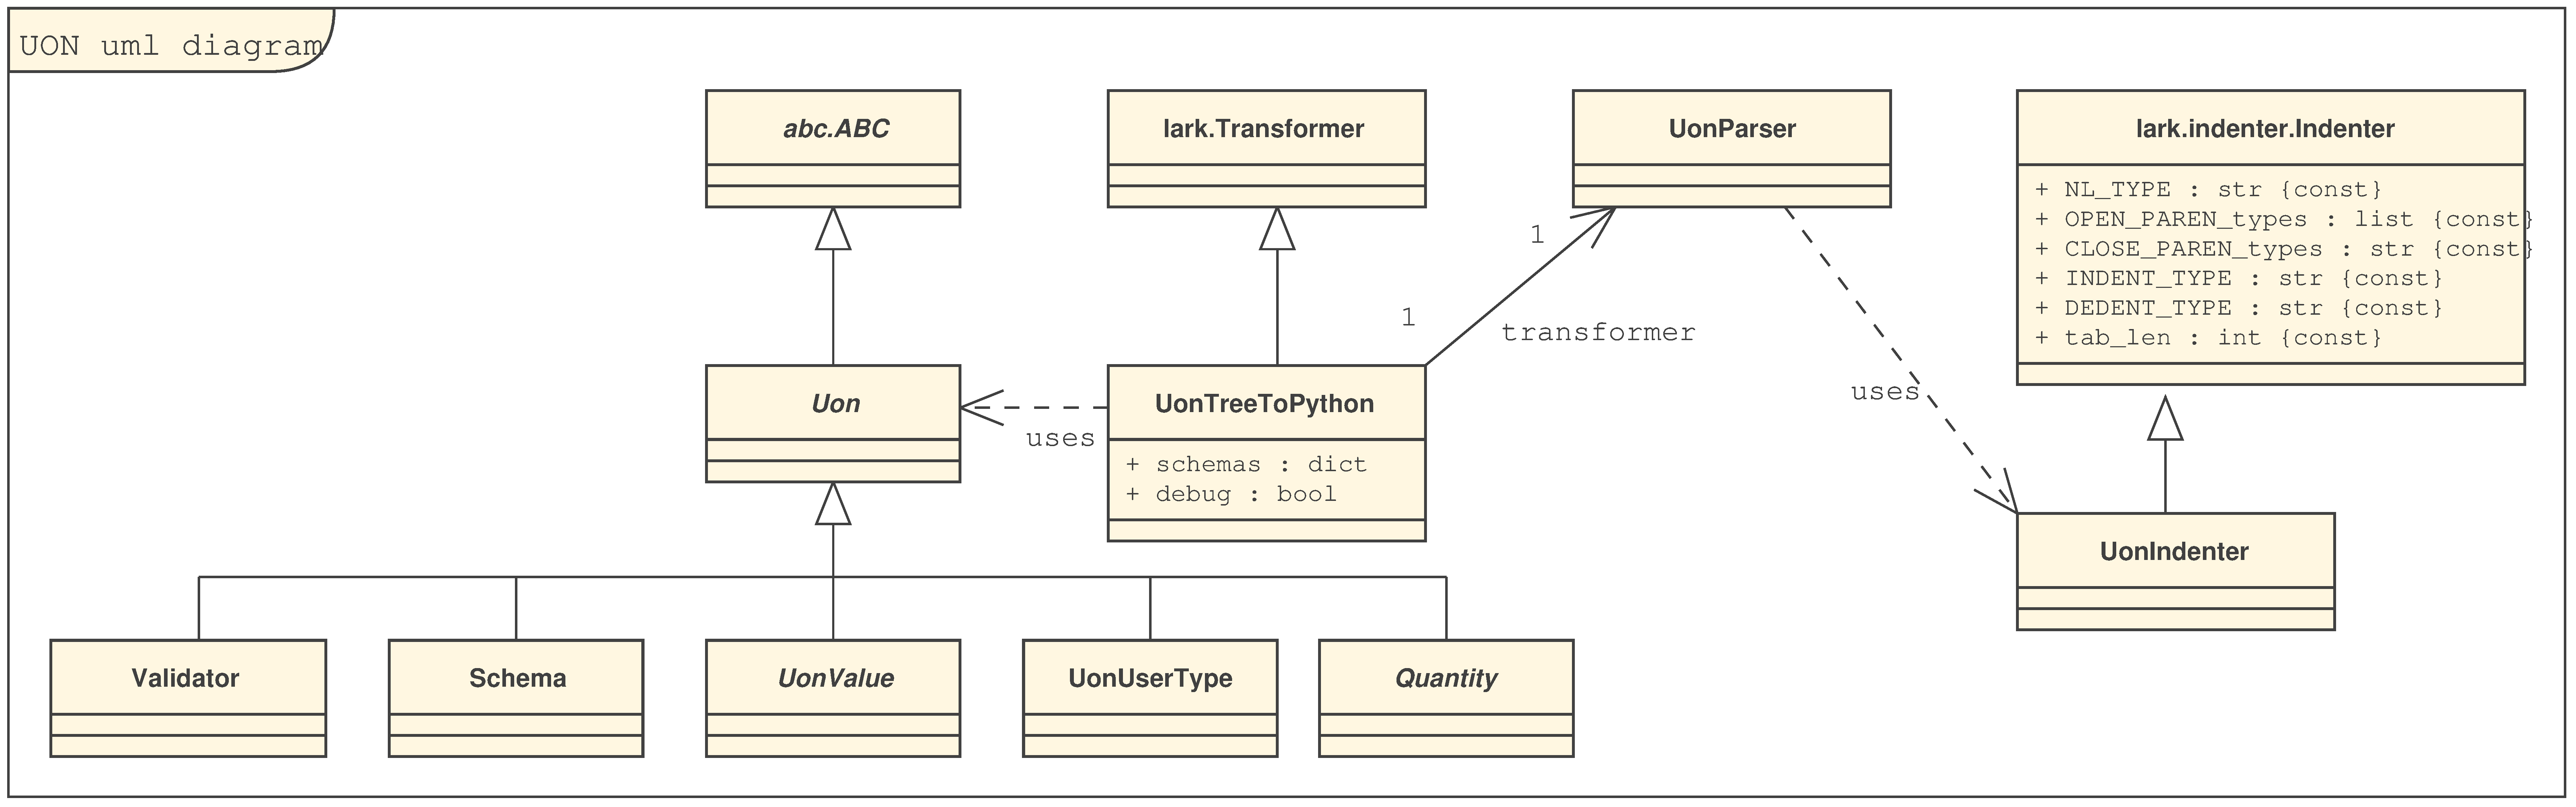
\includegraphics[width=0.9\linewidth]{images/UML/uon_uml.eps}
 	\label{fig:uon_uml}
\end{figure}

This part of the UML diagram shows the base classes comprising our UON parser. The \emph{UonParser} acts as the main interface to our parser, exposing a standard API related to serialization/deserialization, binary encoding/decoding as well as schema validation. Here are the methods if provides:
\begin{itemize}
    \item \emph{load(input)}: parse a raw UON input (string input) and returns the corresponding \emph{Uon} Python object.
    \item \emph{load\_from\_file(input, filename)}: Parses a UON file to \emph{Uon} Python objects.
    \item \emph{load\_schema(schema\_raw)}: Same as \emph{load} but for UON schemas.
    \item \emph{load\_schema\_from\_file)}: Same as \emph{load\_from\_file} but for UON schema file.
    \item \emph{dump(input)}: serialize a Python object to UON.
    \item \emph{dump\_to\_file(input, filename)}: serialize a Python object to UON and dump it to a file.
    \item \emph{to\_binary(uon\_input)}: Given a raw UON input, loads it to a \emph{Uon} Python object and encodes it to binary.
    \item \emph{from\_binary(binary\_input)}: decodes a UON encoded binary input and returns the corresponding \emph{Uon} Python object.
    \item \emph{schema\_from\_binary(binary\_schema)}: Decodes a UON encoded validation schemas and returns the schema Python object.
\end{itemize}

The \emph{Uon} class deriving from \emph{abc.ABC}, Python's abstract class module, defines the base UON type of every UON object. It refers to \emph{!type} in UON's information model \ref{fig:UON information model}. It defines the abstract method \emph{to\_binary} that every deriving concrete UON type has to implement, which is the uon representation of that particular type in binary. Every UON object is a \emph{Uon} object and has its own binary representation that identifies it.

The diagram also shows the classes involved in the parsing and the transformation of the parse tree, namely our transformer \emph{UonTreeToPython} and the \emph{UonIndenter}, inheriting from their corresponding Lark classes. Naturally our transformer has a dependency on \emph{Uon} since it constructs \emph{Uon} objects out of the parse tree when visiting its nodes.

\pagebreak

\subsubsection{Indentation}\label{section:indent}
Before we go any further into the implementation of UON 2, we first have to talk about an aspect of YAML (the syntax of which UON 1 and 2 is based on) : \textbf{indentation}.

What distinguishes YAML from other serialization formats or Python from other Programming languages? It's that indentation matters! It denotes structure just as Python uses it for delimiting blocks and defining scopes. For example:
\begin{lstlisting}
- 
  - Ophelia
- Hamlet
\end{lstlisting}
is equivalent to a nested list inside a list in Python [['Ophelia'], 'Hamlet']
but 
\begin{lstlisting}
- 
- Ophelia
- Hamlet
\end{lstlisting}
is equivalent to just a list of 3 elements in Python [None, 'Ophelia', 'Hamlet']

So indentation is just a bunch of whitespaces (not tabular characters, YAML states that tabs are a source of ambiguities since different systems treat tabs differently). What does that change for our grammar? Unfortunately, it changes everything.

Indentation is context-sensitive. If you're not convinced, ask yourself how does the parser know that "Ophelia" is a nested list in the first example, and not just another list element like in the second example. It's because \textbf{it knows it's surrounded} by an indentation and then a dedentation. That means the result of the parsing is dependent on the context, which here is the indentation.

Denoting blocks using indentation is also called the \textbf{off-side rule}, in contrast to curly-bracket languages where indentation is not meaningful and indent style is only a matter of convention and code formatting (\url{https://en.wikipedia.org/wiki/Off-side_rule}).

How are these off-side rules implemented? In \href{https://docs.python.org/3/reference/lexical_analysis.html#indentation}{Python} this is done during the lexical analysis phase and it usually involves a powerful lexer. When the lexer encounters an increase in indentation, it emits an INDENT token, and when it detects a decrease in indentation, it outputs a DEDENT token. They are the equivalent of opening "\{" and closing braces "\}" when denoting blocks in other languages. However this requires that the lexer hold a state and keep track of the current indentation level. So when it encounters an indentation in the next line, and depending on the current indentation level, it chooses to emit an INDENT or a DEDENT token accordingly. 

\textbf{Handling indentation in Lark}

Fortunately, Lark has a way of handling context-sensitive indentation as well. This involves a postlex stage, where INDENT/DEDENT tokens are manufactured. This means that there two passes, where the first pass is the normal pass of the lexer outputting the tokens according to our grammar, and the second pass concerns the INDENT and DEDENT tokens relevant for indentation. (\url{https://github.com/lark-parser/lark/blob/master/examples/indented_tree.py})

What does that change for our grammar? It means that whitespace and newline suddenly became important and we can't ignore them anymore. And this is going to change the structure of all our grammar.

First we must define what a newline must look like in UON. We define it as such:
\begin{lstlisting}
_NL: /(\r?\n[\t ]*)+/
\end{lstlisting}

Then we declare the INDENT and DEDENT tokens. In lark you can use \emph{\%declare} to declare a terminal in your grammar without defining it. It is useful for plugins or in cases like this one.  

Then you start changing your grammar accordingly. For example for nested collections, we define it as such:

\begin{lstlisting}
_collection: _NL [_INDENT _value _DEDENT]
\end{lstlisting}

A nested collection is defined by a newline followed by an increase in indentation, the value of the collection and then a decrease in indentation to get back to the previous level of indent.

\textbf{Gentle Reminder}: Rules that start with an underscore are inlined in the parse tree.

After adapting our grammar to handle indentation, we must now let our parser know how indentation is done in our language. For that we define our own custom class \emph{UonIndenter} (found in \emph{uon\_tree\_transformer.py}) that inherits from \emph{lark.Indenter} and we must define the following attributes:
\begin{itemize}
    \item \textbf{NL\_type}: the terminal in our grammar that defines how newlines are represented in our language, namely the \emph{\_NL} we've defined above.
    \item \textbf{OPEN\_PAREN\_types} and \textbf{CLOSE\_PAREN\_types}: The indenter takes also the type of enclosing grammatical structures in our language such as parentheses "()", square brackets "[]" or braces "\{\}". In UON, we expect to use every single one of the aforementioned parentheses types, for example we use normal parentheses for describing UON properties, curly braces for defining mappings, and square brackets for defining ranges. So we add them all to the list of \textbf{OPEN\_PAREN\_types} and \textbf{CLOSE\_PAREN\_types} accordingly:
    
    \begin{lstlisting}[language=python]
    OPEN_PAREN_types = ['LPAR', 'LSQB', 'LBRACE']
    CLOSE_PAREN_types = ['RPAR', 'RSQB', 'RBRACE']
    \end{lstlisting}
    
    And what this does is that the parser can safely handle you writing expressions inside enclosing parentheses spanning multiple lines. How this works is that indenter ignores the newline tokens at the end of these lines and the parsing can proceed normally for the expression inside. Here are the first 3 lines of the method \emph{handle\_NL} of \emph{lark.Indenter.py}. 
    
    \begin{lstlisting}[language = python]
    def handle_NL(self, token):
        if self.paren_level > 0:
            return

        yield token
    \end{lstlisting}
    
    It takes a newline token from the lexer (since this is a postlex stage), checks if the current parenthesis level is bigger than 0 which is the equivalent of saying that a parentheses type symbol has been opened and has not been closed yet (same logic for indentation/dedent), and if so it returns from the function, which means there is no newline token emitted that can interfere with the parsing of the expression inside the parentheses and would cause it to fail since a newline token doesn't belong inside the expression. Otherwise, it would just emit the newline token.

    \item \textbf{INDENT\_type} and \textbf{DEDENT\_type}: the terminals in our grammar that represent an indentation or a dedent. In our case, these are the new INDENT/DEDENT tokens that we've declared in our grammar (without defining them).
    \item \textbf{tab\_len}: The length of a tabular character. In our case we define it just for the sake of completeness, but we don't really use, since the use of tabs is discouraged (Different conventions of how many spaces represent a tab).
\end{itemize}

Now we just have to pass this Indenter class to the Lark constructor that generates our parser, to let the parser know that a postlex stage is needed for our language, to handle indentation.

Let's see the result of all this in an example, taken from the YAML spec, where they define a list of two elements, where each element is a mapping of its own:
\begin{lstlisting}[language=Python]
test_indentation = """
-
  name: Mark McGwire
  hr:   65
  avg:  0.278
-
  name: Sammy Sosa
  hr:   63
  avg:  0.288
"""
uon_2_parser = Lark.open(uon_grammar_file, parser='lalr',
                         postlex=TreeIndenter(), start='start', debug=True)
uon_parser_2.parse(test_indentation)
\end{lstlisting}

The result parse tree:

\begin{lstlisting}
top_seq
  seq_item
    top_map
      pair
        pair_key
          string        name
        scalar
          string
            Mark
            McGwire
      pair
        pair_key
          string        hr
        scalar
          number        65
      pair
        pair_key
          string        avg
        scalar
          number        0.278
  seq_item
    top_map
      pair
        pair_key
          string        name
        scalar
          string
            Sammy
            Sosa
      pair
        pair_key
          string        hr
        scalar
          number        63
      pair
        pair_key
          string        avg
        scalar
          number        0.288
\end{lstlisting}

\emph{top\_seq} represent a sequence or a list, and \emph{top\_map} represents a mapping. We can see that our parser recognizes properly the nested maps in our list, by the help of indentation.

So what happens in the case of JSON-like structures in our grammar? Well we don't have to worry since there is no indentation involved. Moreover, the modifications we made to the grammar don't have an effect on JSON-like structures because JSON structures are enclosed inside braces and braces are enclosing type parentheses in our Indenter. Thus any newline token or whitespace inside JSON-like structures are ignored and won't interfere with the parsing.
\pagebreak

\subsection{Transforming UON to Python}
To be able to transform our UON parse tree to Python, we need to be able to represent the different UON native data types in Python. We could directly translate these different UON types into the closest equivalent data type in Python, for example a UON float into a Python \emph{float}, a UON string into a Python \emph{str}, a mapping into a Python \emph{dict} and so on...

But this approach is too restrictive. UON objects have much more information to them than just their value and that could not be simply represented by a Python native data type. One information that comes to mind is their binary representation. Each object type in UON has its own custom UON binary encoding and it would be nice to have a method for each type that just returns its corresponding binary representation in an Object-Oriented style, and that's what we did when we defined the base type \emph{Uon}.

UON types are not all similar either, each has information endemic to their type or meaning. For example a UON numeric has its precision, a UON sequence has its size (the number of elements). 

This problem will only become clearer when we're implementing schema validation later on, because as far as we're concerned, Python does not have an equivalent in-built data type to represent schemas.

So the idea was to wrap a UON value in a Python object and then extend it with new functionalities. Each UON object type has its own class in Python, and for the following we will implement those that represent a value, having type \emph{UonValue} subclass of base type \emph{Uon} which we've already encountered when we presented the general UML diagram \ref{fig:uon_uml}, where it was collapsed for the sake of visual clarity. Here we present the full \emph{UonValue} class hierarchy of the types that we've implemented. \textbf{Note that not all types found in the specification were implemented}, for example there are no ordered maps or sets data structures, only the most basic of types, that could help build other types, have been implemented (as a proof of concept).

\begin{figure}[ht!]
 	\centering
 	\caption{UonValue class diagram}
 	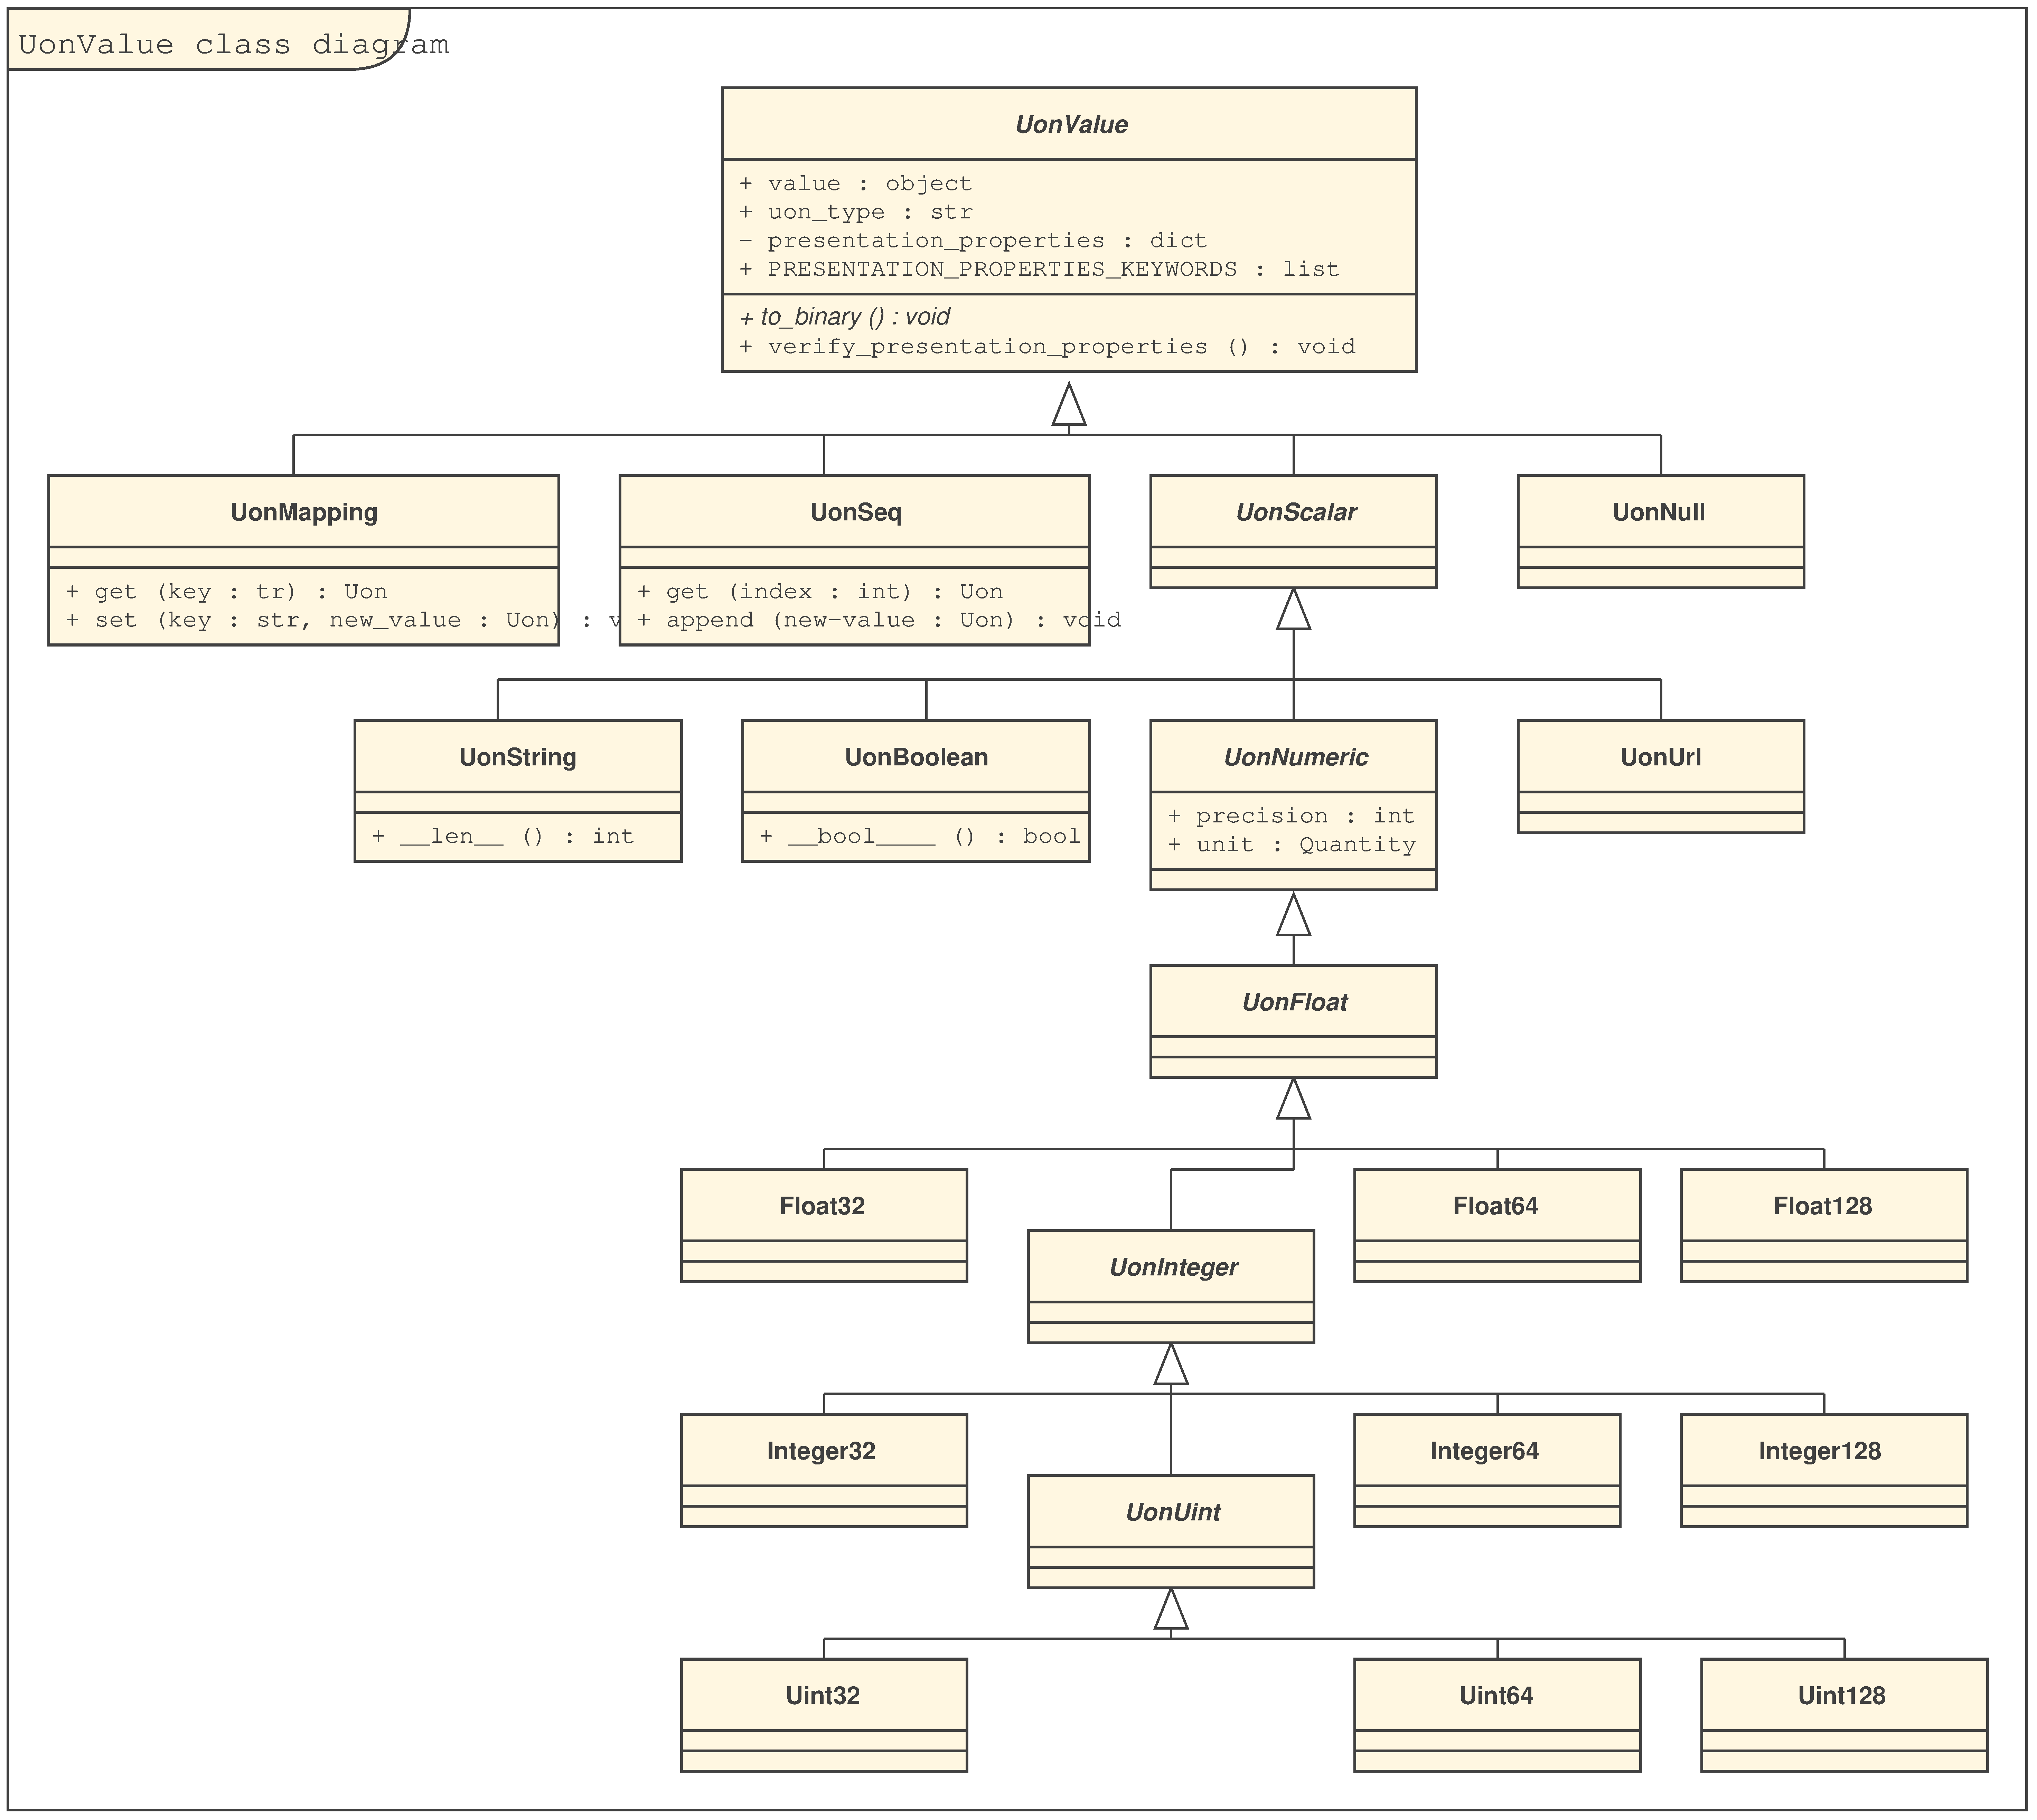
\includegraphics[width=0.9\linewidth]{images/UML/uon_value.eps}
 	\label{fig:uon_value_uml}
\end{figure}

Every \emph{UonValue} has a \emph{value}, which is the equivalent data type in Python of that value. This is the fundamental characteristic of a \emph{UonValue}, \textbf{it encapsulates a value}. A \emph{UonValue} also has \emph{uon\_type} which is string representation of the type in UON (which will be useful when serializing back to UON),  as well as presentation properties that we've already seen like \emph{description} or \emph{optional}. For now, only these two properties are implemented.

A \emph{UonValue} can be a scalar value (\emph{UonScalar)} or a compound value of other \emph{UonValue}s (collections). It can also be \emph{UonNull} (absence of value).

The implementation of \emph{UonValue} and its class hierarchy can be found in the package \emph{uontypes}.

\pagebreak

\subsubsection{UonString}
UON string are represented by \emph{UonString}. Its attribute \emph{value} is a Python string (\emph{str}). 

Strings in UON do not have to double quoted. However, you can still double quote them or single quote them quite like in Python. However you cannot triple quote them to form multiline strings, multiline strings will be handled differently as we will see shortly.

How do we parse strings in our grammar? The first issue is that whitespace is ignored in our grammar, that is it doesn't appear as tokens in the parse tree (it is discarded already by the lexer). So we can't use regular expressions to parse whole strings because the whitespace characters won't be there.

A string is made up of words and punctuation just like a sentence. So first we can define what a word is:

\begin{lstlisting}[label={grammar:word}]
WORD: /[^\n\"\'\s]+/
\end{lstlisting}

We used the negated set notation in regular expressions "[\textasciicircum" to include everything except what's inside the brackets, namely whitespaces ("\textbackslash s") and newlines ("\textbackslash n") given how important they are as separators in my UON 2 grammar for YAML-like structures. We don't want a newline to be mistaken for a word or as a part of a word, then there would be no newline token after to separate between two pairs in a YAML mapping.

The problem with this approach is that it will match punctuation as well and that could cause ambiguities and would not really represent a real word. A real sentence starts with a word and is intertwined with punctuation. The second problem is that some punctuation have special meanings in our grammar. For example commas "," separate between pairs of a mapping in JSON, properties such as description and optional are inside brackets "()"... So if we take this simple json example:

\begin{lstlisting}[language=Python]
{
    a: hello,
    b: world
}
\end{lstlisting}

The comma following hello will be eaten as part of the word according to our WORD rule and there will be no more comma to separate the two pairs a and b, resulting in a parse error.

So an idea was to naturally separate punctuation from words:

\begin{lstlisting}

escaped_string : "\"" unescaped_string "\"" | "'" unescaped_string "'"
unescaped_string: WORD (WORD | PUNCTUATION)*
WORD:  /[^:#,()\[\]{}!?\n\"\'\s]+/
PUNCTUATION: /[:#,()\[\]{}!?\"\'\]/
\end{lstlisting}

We refer to quoted strings as \emph{escaped\_string} and we refer to those that aren't as \emph{unescaped\_strings}. However the problem of the last example still persists. Unless the string is between quotes, the comma at the end of "hello," will be considered part of the word. So we have to modify the punctuation allowed depending on if we're dealing with \emph{escaped\_strings} or \emph{unescaped\_strings}. A string that isn't quoted \textbf{CANNOT end with commas}. We have to reinforce this rule to avoid any ambiguities, especially from the user input. We don't want a user to be able to input something like 
\begin{lstlisting}[language=Python]
{
    a: hello, ,
    b: world
}
\end{lstlisting}

and expect the first comma to be parsed as part of the string "hello,", and the second to be parsed as the separator betweens the pairs a and b in the mapping.

Worse yet to be able to parse something like this :
\begin{lstlisting}[language=Python]
{
    a: hello : world ,
    b: world
}
\end{lstlisting}
The ambiguity is obvious here. The colon ":" acts as separator between key and value in a mapping. So is the key in that example "a: hello" or just "a"? The colon is removed from the set of allowed punctuation for \emph{unescaped\_string}.

So the grammar for strings becomes roughly.

\begin{lstlisting}
_string: escaped_string | unescaped_string | multiline_string
escaped_string : "\"" _escaped_string_helper? "\"" | "'" _escaped_string_helper? "'"
_escaped_string_helper: WORD (WORD | PUNCTUATION)*
unescaped_string : _unescaped_string_helper
_unescaped_string_helper :  WORD (WORD | UNESCAPED_PUNCTUATION)*

WORD:  /[^:#,()\[\]{}!?\n\"\'\s]+/
PUNCTUATION: /[:#,()\[\]{}!?\"\']/
UNESCAPED_PUNCTUATION: /[#?!\"\'()\[\]]/
\end{lstlisting}

\textbf{Note} that this is one solution and there may exist others that involve playing with the grammar, but in the end whichever solution we choose to implement, it must ensure a grammar that is unambiguous for the parser and for the user. 

It's clear that our strings' regular expressions still need reworking and fine-tuning, but for now they should do the job.

Finally, we need to parse multi-line strings. In the case of JSON-like structures, strings inside can span over multiple lines without any problem since there is no newline involved in the parsing of JSON. However, in the case of YAML-like structures, this can become a problem. Whitespace between words is ignored but not newline tokens, which are parsed and will figure among the words of a string, which will in turn cause a parsing error since newline characters are among the characters that are not allowed in our negated set of characters for a word (nor punctuation) \ref{grammar:word}. How do we solve that?

Remember the enclosing type parentheses that we discussed in the indentation \ref{section:indent}? Newline tokens are ignored inside these structures. So we can enclose our strings in these structures if we want them spanning multiple lines without having to worry about the newline tokens. In our case, multiline strings are enclosed within parentheses as such:
\begin{lstlisting}
multiline_string: "(" (unescaped_string | escaped_string) ")"
\end{lstlisting}

So if we test it:
\begin{lstlisting}[language=Python]
test_multiline_simple = """
multiline-line: (I'm writing a very 
loooooooooooooooooooooooooooooooooong
string)
"""
\end{lstlisting}

we get:
\begin{lstlisting}
multiline_string
          unescaped_string
            I
            '
            m
            writing
            a
            very
            loooooooooooooooooooooooooooooooooong
            string
\end{lstlisting}

No newline tokens and the string has been successfully parsed. In conclusion, \textbf{to write multi-line strings, you have to enclose them with parentheses} (a feature present in Python as well, which served as inspiration here).

\textbf{Persistent problems when parsing strings} \\

A persistent problem in our parser regarding strings is keeping white space information in the parse tree. Languages often ignore whitespaces since they can come anywhere because it would be easier to ignore them than to add them before and after each and every rule or terminal (basically everywhere in our grammar), when they provide no additional semantic information apart from acting as separators between the tokens of our grammar. So how does that reflect in parsing our strings? Well if we have 2 or more whitespaces between 2 words in a string, they will not be parsed and we will lose that information. Strings are formed during post-parse(transformation) by joining them with a single whitespace separator:

\begin{lstlisting}[language=Python]
def unescaped_string(self, string):
        s = ' '.join(string)
        return UonString(s)
\end{lstlisting}

That's why an example like "Hello \hspace{1cm} (world)" will be transformed into "Hello ( world )". Note how only one whitespace character is separating our words and punctuation.

\subsubsection{UonNumeric}
UON aims to support a large number of numeric data types with different precisions. \href{https://github.com/uon-language/specification/blob/master/spec.md#numbers-datatypes}{See the specification for the available numeric datatypes}.

For the following, we implement only the single (32 bit) and double (64 bits) precision for the different numeric data types. But it can easily be extended with short (16 bits) and single-byte precision (8 bits) following the same workflow. We focus on the two aforementioned precisions as a proof of concept. We also implement the classes for 128 bits precision numeric data types, but they are only experimental and have not been tested.

The class hierarchy for the \emph{UonNumeric} classes (See \ref{fig:uon_value_uml}) roughly follows that of the UON specification. First there are \emph{Float}s which in reality are what we refer to as decimal real in the specification. Then there are the \emph{Integer} classes that subclass \emph{Float}. And finally the unsigned integers \emph{Uint} that subclass \emph{Integer}. 

To store the actual numeric value, we use the excellent \emph{numpy} library, that provides support for most of the numeric data types that we're after. \emph{Numpy} provides constructors for these different data types e.g. \emph{numpy.int64()} or \emph{numpy.float32()}. You can also specify the data type as a kwarg \emph{dtype} in a numpy constructor (e.g. np.ndarray(shape=(2,2), dtype=float64)). \emph{Numpy} constructors are also able to parse numbers from their string representation.

As well as the numeric value, we provide the additional information of \emph{precision} and \emph{uon\_type} for each \emph{UonNumeric} data type.

So how do we parse numbers in the grammar? The numbers will be parsed in the grammar as strings using regular expressions, and then parsed to numbers using the numpy constructors.
\begin{lstlisting}
number : decimal | signed_decimal | float_number
decimal : DECIMAL
float_number: FLOAT_NUMBER
signed_decimal: "-" DECIMAL

DECIMAL : /0|[1-9]\d*/i
FLOAT_NUMBER: /((\d+\.\d*|\.\d+)(e[-+]?\d+)?|\d+(e[-+]?\d+))/i
\end{lstlisting}

It is pretty straightforward. However, there's a problem with this. Let's try and test it with a simple example:
\begin{lstlisting}[language=Python]
test_simple_number = """
c : 3
"""
\end{lstlisting}

\begin{lstlisting}
pair
    pair_key
      unescaped_string  c
    string_scalar
      unescaped_string  3
\end{lstlisting}

It interpreted the -3 as a string!

If we look at how we defined a \emph{WORD} token (\ref{grammar:word}), we see that it includes any characters including digits. So there's an ambiguity there, a number like 3 satisfies both regular expressions \emph{WORD} and \emph{DECIMAL}. So why does Lark choose to parse a WORD instead of a DECIMAL? 

Lark has lexer priorities where you can assign priorities to Lark grammar terminals. That means that when lexing our input, the lexer will match the terminal with the highest priority first. If not specified for a terminal, a terminal has a priority 1 by default (the lowest). So our \emph{WORD} and our terminals that constitute the production rules for our number, namely \emph{DECIMAL} AND \emph{FLOAT\_NUMBER}, all have the same priority. What happens if the lexer meets an input literal like “3” and priorities of WORD and the number terminals match? It will match the literal according to the following precedence:
\begin{enumerate}
    \item Highest priority first (priority is specified as: TERM.number: ...)
    \item Length of match (for regexps, the longest theoretical match is used)
    \item Length of literal / pattern definition
    \item Name
\end{enumerate}

So when it comes down to \emph{WORD} terminal or \emph{DECIMAL} terminal, they both have the same default priority 1, however the length of match for \emph{WORD} is longer than that of \emph{DECIMAL}, so \emph{WORD} gets matched first. If we try and test between \emph{FLOAT\_NUMBER} and \emph{WORD}, \emph{FLOAT\_NUMBER} wins and it gets matched rather than \emph{WORD}, since \emph{FLOAT\_NUMBER} has the longest match.

So how do we solve the ambiguity between \emph{DECIMAL} and \emph{WORD}. Should we lenghten the regex that describes \emph{DECIMAL}? We can't do that, it's already at its minimal and sufficient form of regular expression, and it would be forcing the grammar too much. We can increase the priority on the \emph{DECIMAL} rule so that it would always parse a \emph{DECIMAL} before a \emph{WORD} or a \emph{FLOAT\_NUMBER}. But this doesn't make sense in the grammar semantically (why would a decimal have more priority than a float number?) and it would introduce a problem when parsing a float number or strings that start with a decimal, since that decimal will be parsed as a \emph{number} directly, and the parse will fail on the rest of the inputs.

For example, with \emph{DECIMAL}'s priority set higher, parsing the following:
\begin{lstlisting}[language=Python]
test_simple_number = """
c : 3.2
"""
\end{lstlisting}
will fail. The input is obviously a \emph{FLOAT\_NUMBER} but, since \emph{DECIMAL} has priority, the "3" before the decimal point will be parsed directly as a \emph{number} consisting of a \emph{DECIMAL}, and the parse will fail on the rest of the input ".2" since there is no rule describing a number followed by a decimal point and other digits.

The same will happen, if a string starts with a decimal number, the decimal number will be parsed first as a number, and the parsing will fail on the rest of the input since there are no rules describing a number followed by words.

\textbf{The Solution} \\
After discussing the matter on the Lark forum on Gitter and as per the suggestion of the author of Lark, it would be better to keep the grammar as is and instead “disambiguate post-parse. Increasing the priority on the number will cause strings to be misidentified as numbers, because the parser can’t see what comes after”, which as we've seen is exactly what happened. Disambiguate post-parse in this case means checking when transforming the string if the string is a number (incorrectly interpreted as a string) or not.

So we add an additional grammar rule \emph{string\_value}:
\begin{lstlisting}
string_scalar: [STR_TYPE] string_value

string_value: _string
_string: escaped_string | unescaped_string | multiline_string
\end{lstlisting}

In the transformer for this rule, we check if the string represents a number by trying to parse it. If the parsing passed, then the string is a number and we convert it to the corresponding number data type. If it throws an exception, then input is not a number, it's a normal string.

\begin{lstlisting}[label=transformer:string_value]
@v_args(inline=True)
    def string_value(self, string):
        value = string
        # Check if it's an integer
        try:
            value = int(string.value)
            value = Integer64(value)
        except ValueError:
            # Check if it's a float instead
            try:
                value = float(string.value)
                value = Float64(value)
            except ValueError:
                pass
        return value
\end{lstlisting}

Although it might not look clean, it's a valid workaround since numbers are passed from the lexer to the parser as tokens (strings) anyway, and some parsing would be involved at some point to transform these tokens into actual number data types. This way we also keep the grammar syntactically and semantically intact. Every rule represents clearly and precisely what it should parse, no more no less.

\textbf{Persistent problems in parsing \emph{UonNumeric}}
We are still left with the problem of parsing a string that starts with a float, since as mentioned before, \\ \emph{FLOAT\_NUMBER} terminal has higher precedence than \emph{WORD} terminal and the float at the beginning will be parsed as a float and not a word. The only way to do so it is to force the string to be a string by adding the "!str" type before the string itself. That way the grammar will see that it starts with a \emph{STR\_TYPE} and expects the following to be a string. This extends to all other types as well. 

Another problem with disambiguating between decimal numbers and strings post-parse, that appeared in later stages of development when we incoporated units and quantities into \emph{UonNumeric}, is parsing numbers that are followed by units that denote a quantity like temperature. For example, the \emph{UonNumeric} here denotes a temperature value of 32 Kelvin:
\begin{lstlisting}[language=Python]
temperature : 32 K
\end{lstlisting}
These units are letters or words. Naturally, they will be included in the string that is passed on to \emph{string\_value()} (\ref{transformer:string_value}) transformer method that checks if it really corresponds to a string or rather a number. So when passing the value to an integer or float constructor, the parsing will fail since it doens't recognize unit characters and the output will still be a string, even though in reality it denotes a \emph{UonNumeric} with a unit. We can try to add more fine handling of the input to check if characters appear after the number, and figure out if they denote units, but this is cause for ambiguities and is not a very sustainable solution as more quantites or units are added in the future. The best solution here should come from the user by again forcing the type of the \emph{UonNumeric} by adding a number type before the value, for example:
\begin{lstlisting}[language=Python]
temperature : !uint32 32 K
\end{lstlisting}

\textbf{It's now a general best practice} from here on out: to make sure that your input corresponds to the type you want it to be in UON, precede it explicitly with that type (using "!" for native UON types, or "!!" for user-defined types, that we'll discuss later on).

\subsubsection{UonMapping}
A mapping in UON is a collection of keys mapped to their values. UON mapping are implemented in the \emph{UonMapping} class, encapsulating a value of type \emph{dict} in Python. It defines standard dictionary API methods to \emph{get()} and \emph{set()} on the dictionary value it encapsulates.
 
We will build on the JSON example of section \ref{grammar:json} to parse mappings. For JSON-style mappings we keep the same structure:
\begin{lstlisting}[label=grammar:uon_json]
json_mapping : [MAPPING_TYPE] "{" [json_pair ("," json_pair)*] "}"
json_pair: pair_key ":" _json_value

_json_collection: json_mapping | json_seq
_json_value: _scalar | (_json_collection _NL*) | json_user_type | null

pair_key : unescaped_string [presentation_properties]

presentation_properties : "(" [_presentation_property ("," _presentation_property)*] ")"
_presentation_property : optional | description
\end{lstlisting}
So a JSON mapping is a list of pairs, preceded by an optional !mapping type. The JSON value can be a scalar value or another collection, which in this case will be nested. Here's how we transform the parse tree of a mapping:

\begin{lstlisting}[language=Python, label=grammar:mapping]
def json_mapping(self, mapping):
        return UonMapping(
            UonTreeToPython.to_dictionary(mapping))
            
@v_args(inline=True)
    def json_pair(self, key, value):
        """
        We receive a key pair inside a (key, value) pair. Expanded, we have
        ((keyname, presentation_properties), value).
        The presentation_properties are "transferred" to be part of the
        UonValue.
        We return a pair (key, UonValue) with the key being the 
        keyname (a string).
        """
        key, presentation_properties = key
        v = value
        v.presentation_properties = presentation_properties
        return key, v
        
@staticmethod
    def to_dictionary(tuples_list):
        """
        Construct a dictionary out of a list of tuples.
        The 1st element of the tuple serves as key and the second
        is the value. Throws an error if a duplicate key was found.
        """
        d = {}
        for k, v in tuples_list:
            try:
                d[k]
                # If d[k] passed, then a key with the same name exists.
                raise UonDuplicateKeyError("Key {} already exists".format(k))
            except KeyError:
                # Didn't find the key in the dictionary. We can add it.
                d[k] = v
        return d
\end{lstlisting}

In the parse tree, the presentation properties of a \emph{UonValue} are part of the key since in the grammar they are located on the key side of a pair (before the colon ":"). So first the presentation properties are "transferred" to the value. A JSON pair is parsed and returned as a tuple. 

The \emph{json\_mapping} will thus receive a list of tuples from all of its children pair nodes, which is very convenient since in Python you can construct a \emph{dict} from a list of tuples. But the Python \emph{dict} constructor doesn't check for duplicates, and will automatically override the value of an existing key with the value of the last duplicate found. While in UON, we should logically return an error if duplicate keys were found in a mapping. So to construct the dictionary, we define a helper static method \emph{to\_dictionary} where we have to go manually checking at every update if the key already exists, and if it does we return a custom-defined \emph{UonDuplicateKeyError} exception. We thus sacrifice the convenience of plugging in the list of pairs we receive from the children nodes, directly to the \emph{dict} constructor.

It was very important since the start for UON mappings keys to have:
\begin{enumerate}
    \item keys that are hashable. Keys need to be hashable to be able to build a dictionary in Python.
    \item keys that are easily searchable: for example strings or numbers.
\end{enumerate}
At first, the keys were parsed as \emph{UonString}s since in the \emph{pair\_key} rules that defines them, they use the string rules and these are transformed into \emph{UonString}. \emph{UonString} is easily hashable (we only need to hash the string value it encapsulates), however it is very inconvenient when searching the dictionary, since each time we need to build a \emph{UonString} object encapsulating the key string that we're searching for. So we decided that we needn't encapsulate the key in a \emph{UonString} at all, we only need to keep its value: the key itself (the actual string). So when transforming a \emph{pair\_key}, we made sure to only keep the string value of the \emph{UonString} key:

\begin{lstlisting}[language=Python]
@v_args(inline=True)
    def pair_key(self, key, presentation_properties):
        if presentation_properties is None:
            presentation_properties = {}
        return key.value, presentation_properties
\end{lstlisting}

We were also careful to choose to parse the keys only as unquoted strings (\emph{unescaped\_string} rule in the grammar) to avoid key strings with escaped quotes.

The same logic follows when parsing YAML-like mappings, except that we have to deal with indentation and newlines in YAML collections.
\begin{lstlisting}[label=grammar:uon_yaml]
yaml_mapping :  [MAPPING_TYPE]  pair+
_yaml_collection: yaml_mapping | yaml_seq
pair: pair_key ":" _yaml_value
_yaml_collection_nested: _NL [_INDENT _yaml_collection _DEDENT]
yaml_user_type: _custom_type _NL _INDENT yaml_mapping _DEDENT
_yaml_value: _scalar _NL+ | _yaml_collection_nested | yaml_user_type | null _NL+
\end{lstlisting}

Compared to JSON style mappings, the pairs of a YAML mapping need not be separated with commas (","), they only need to be separated by newlines, or indentations in the case of nested collections (Newline -> Indent -> nested collection -> dedent).

\textbf{Note:} The initial design of the \emph{UonMapping} class aimed to have it be more than just a wrapper for the Python \emph{dict} object, but to be a dictionary object itself, that is deriving from \emph{dict}. So when looking into how to override a dictionary, I stumbled upon the abstract base classes (abc) module of Python, the same from which we derived our base abstract \emph{Uon} type. abc offers a \href{https://docs.python.org/3/library/collections.abc.html}{module} \emph{collections.abc} that "can be used to test whether a class provides a particular interface; for example, whether it is hashable or whether it is a mapping." One such interface is the \emph{MutableMapping}.

An example of such custom implementation \href{https://stackoverflow.com/questions/21361106/how-would-i-implement-a-dict-with-abstract-base-classes-in-python}{found on Stack Overflow}, and extended with UON would be like: 
\begin{lstlisting}[language=Python]
from collections.abc import MutableMapping
from uontypes.uon_value import UonValue

class UonDictionary(MutableMapping, UonValue):
    '''
    Mapping that works like both a dict and a mutable object, i.e.
    d = D(foo='bar')
    and 
    d.foo returns 'bar'
    '''
    # ``__init__`` method required to create instance from class.
    def __init__(self, *args, **kwargs):
        '''Use the object dict'''
        self.__dict__.update(*args, **kwargs)
    # The next five methods are requirements of the ABC.
    def __setitem__(self, key, value):
        self.__dict__[key] = value
    def __getitem__(self, key):
        return self.__dict__[key]
    def __delitem__(self, key):
        del self.__dict__[key]
    def __iter__(self):
        return iter(self.__dict__)
    def __len__(self):
        return len(self.__dict__)
    # The final two methods aren't required, but nice for demo purposes:
    def __str__(self):
        '''returns simple dict representation of the mapping'''
        return str(self.__dict__)
    def __repr__(self):
        '''echoes class, id, & reproducible representation in the REPL'''
        return '{}, D({})'.format(super(D, self).__repr__(), 
                                  self.__dict__)
    def to_binary(self):
        return b"\x00"
\end{lstlisting}

This allows us to very conveniently access the dictionary keys like attributes, like we do with mutable objects. For example:
\begin{lstlisting}
>>> d = UonDictionary()
>>> d['a'] = 3
>>> d.a == d['a']
>>> True
\end{lstlisting}

However what happens when the dictionary object has a key that clashes with the name of one of this methods? For example:
\begin{lstlisting}
>>> d = CustomDictionary()
>>> d['a'] = 3
>>> d['to_binary'] = 4
>>> d.to_binary()
>>> TypeError: 'int' object is not callable
\end{lstlisting}

The previous example returns a type error since d.to\_binary would return 4 (and not our function \emph{to\_binary()}) which is not a callable function.

That's \href{https://stackoverflow.com/questions/4984647/accessing-dict-keys-like-an-attribute}{one reason Python doesn't provide this functionality out of the box:} it combines the namespace of stored keys (which may come from arbitrary and/or untrusted data!) with the namespace of builtin dict method attributes, or in our case with the namespace of any method we add to the class.

It would have been a nice-to-have feature, but at the end we chose to keep the \emph{UonMapping} as a wrapper for an encapsulated \emph{dict} attribute, to avoid this problem and to be on a par with the other \emph{UonValue} classes of the hierarchy. At the end, the defining trait of a \emph{UonValue} is that it encapsulates a value and in the case of \emph{UonMapping}, it encapsulates a Python \emph{dict}.

\subsubsection{UonNull}
To express null values in UON, we create the corresponding class \emph{UonNull} which doesn't hold any value. Since null literally means the absence of value, we cannot inherit the class from \emph{UonValue}. So we inherit it from the base type \emph{Uon} instead.

In the grammar, we choose to have them \textbf{explicitly} expressed as "null" or "none". There is no syntactic sugar as stated in the specification or in YAML, where you can just leave the value empty and pass on to the next pair or element. This will risk ambiguity, because the parser doesn't know if it's a real null value, or just an error from the user who forgot to plug in a value. In any case the parser will take the next token as the value, and this will cause parse errors. For example:
\begin{lstlisting}[language=Python]
{
    a: ,
    b: 3
}
\end{lstlisting}

The parser will look at the token after the colon, in this case the comma "," and will take it as the value of the pair. However when looking for the comma separating the two pairs in the JSON dictionary, it will not find it since it has been parsed as a value for key 'a'. 

This also means that if you want to input an empty string, you have no other way but to use double quotes "" explicitly.

\subsubsection{Quantities and Units}
An important information for telemetry systems and the Internet of Things is the unit of magnitudes. When transmitting a temperature, it is essential to know which unit is used to represent that number. UON aims to add native support for units and quantities, something that not a lot of serialization formats do.

Quantities and units only make sense when it's about numeric values. So in our grammar, units cannot be preceded with a string or a boolean value for example. 

\begin{figure}[ht!]
 	\centering
 	\caption{UON quantity and units}
 	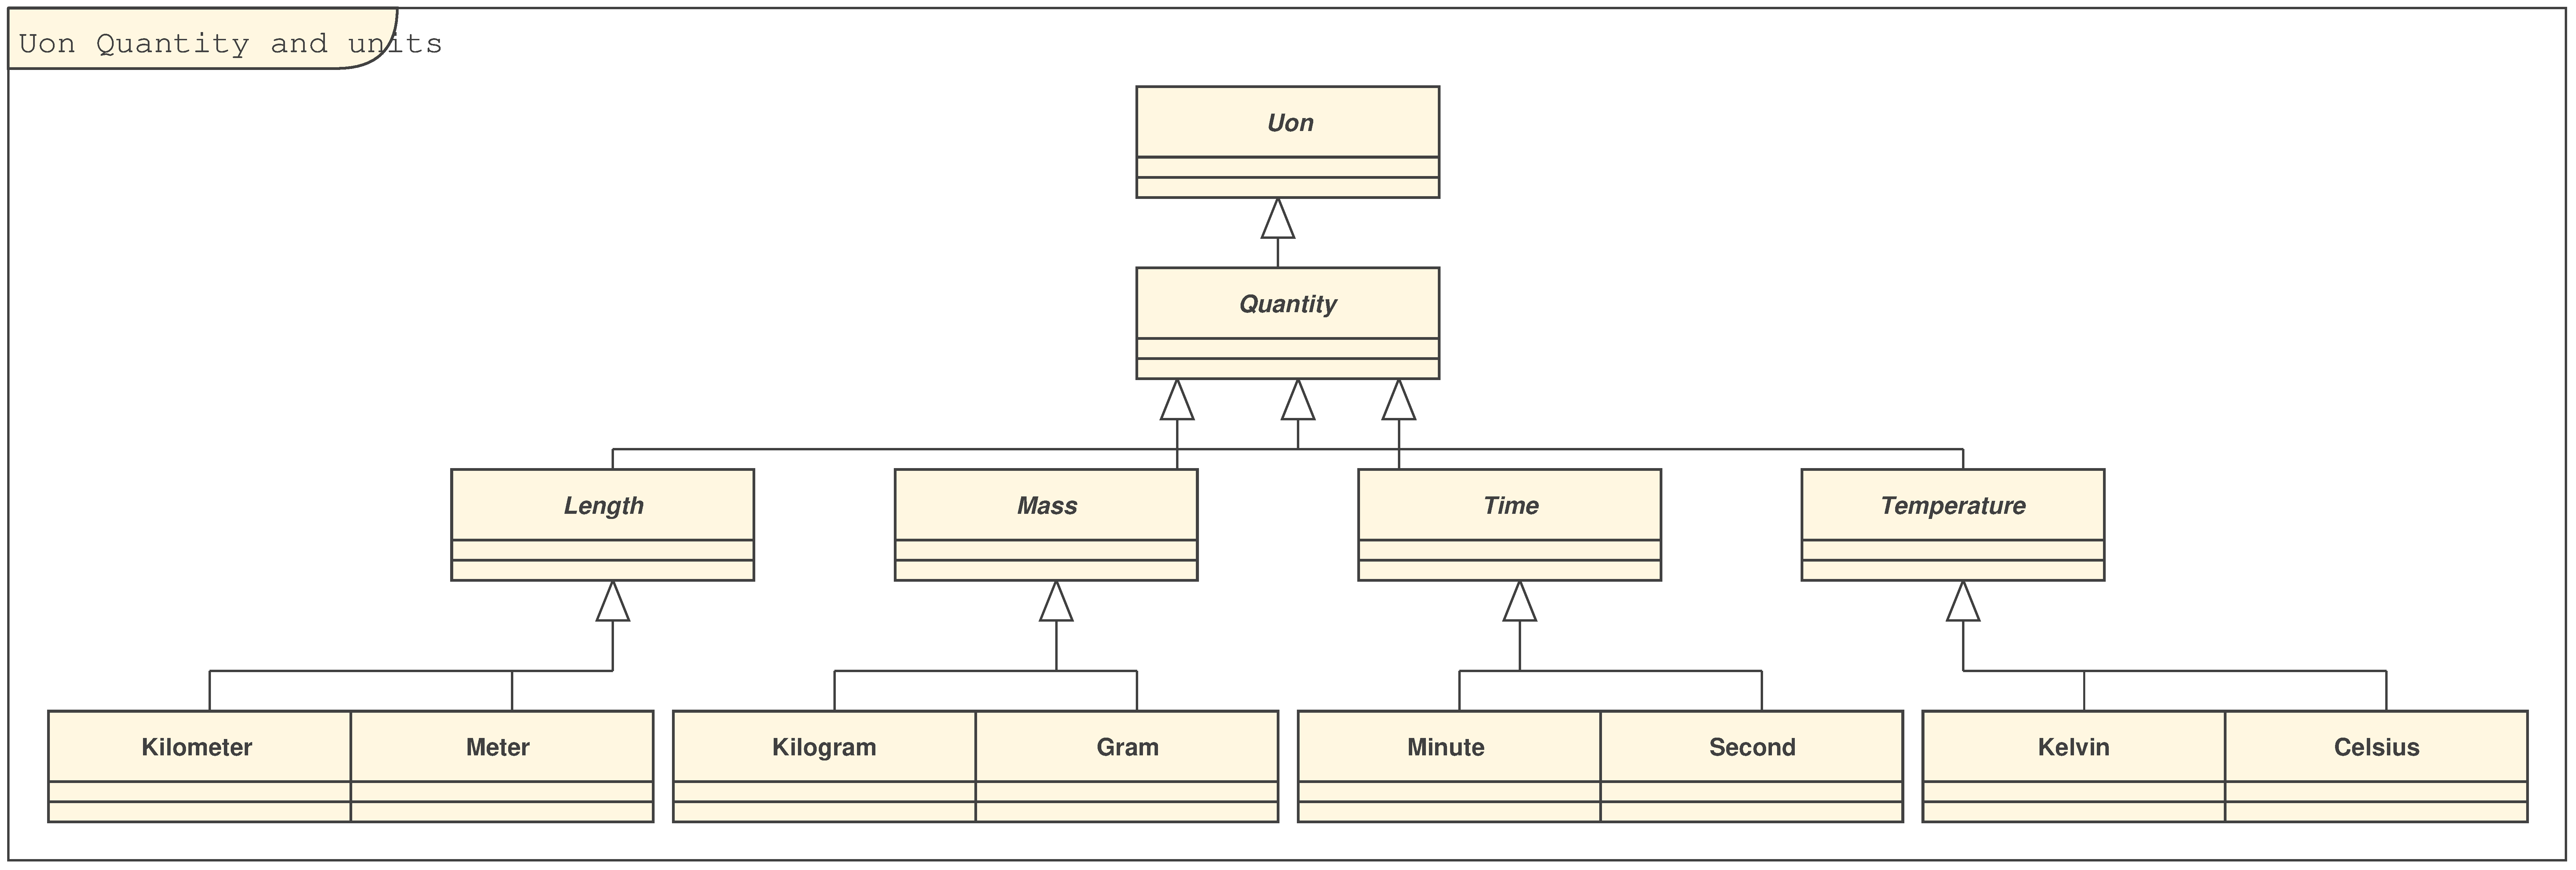
\includegraphics[width=1.0\linewidth]{images/UML/uon_units.eps}
 	\label{fig:uon_units_uml}
\end{figure}

To represent quantity and unit, we first add the quantity unit as an attribute to our \emph{UonNumeric} classes (see UML diagram \ref{fig:uon_value_uml}). Then we establish a class hierarchy for units \ref{fig:uon_units_uml}. We don't implement all the quantities and units stated in the UON specification, We only focus on the smallest functioning subset again as a proof of concept which is easily extendible. Neither one of \emph{Quantity} or any of the subclasses have any attributes regarding units. Instead, the class itself represents the information we need. Since the class itself doesn't hold any value, we cannot inherit from \emph{UonValue}. However each concrete \emph{Quantity} class has its own binary encoding, so it inherits from base type \emph{Uon} directly. (See UON general class diagram \ref{fig:uon_uml})

Then in the grammar we plug them in directly in the numeric scalars:

\begin{lstlisting}[language=Python]
_scalar : quantity_scalar | string_scalar | boolean_scalar | url
quantity_scalar: [number_type] number [quantity]

quantity: length | mass | time | temperature

length: METERS | KILOMETERS
METERS: "m"
KILOMETERS: "km"
\end{lstlisting}

So a numeric scalar now becomes a quantity scalar: a numeric scalar followed by an optional quantity. So overall, a \emph{quantity\_scalar} becomes an optional explicit numeric type, followed by the numeric value, followed by an optional quantity. Let's take a look at what this translates to in the corresponding transformer method in \emph{uon\_tree\_transformer.py}:

\begin{lstlisting}[language=Python]
@v_args(inline=True)
    def quantity_scalar(self, number_type, number, quantity):
        # OMITTED PART: Construct the UonNumeric object corresponding the number_type
        numeric_scalar.quantity = quantity
        return numeric_scalar
        
    grams = lambda self, _: Gram()
    kilograms = lambda self, _: Kilogram()
    meters = lambda self, _: Meter()
    kilometers = lambda self, _: Kilometer()
    kelvin = lambda self, _: Kelvin()
    celsius = lambda self, _: Celsius()
    second = lambda self, _: Second()
    minute = lambda self, _: Minute()
\end{lstlisting}

However there's one problem with this naive implementation. The transformer method for \emph{quantity\_scalar} inlines the arguments of the children nodes it receives using \emph{v\_args}. But what happens if quantity isn't there (since it's optional)? One thing to remember about the Lark parser, is that if it doesn't find the value, it doesn't replace it by default with a null value in the parse tree. The child node just isn't there and won't appear in the parse tree. So we will be receiving two arguments instead of 3 and this will cause an error in the transformation.
\hfill\break

\textbf{Improving the transformer} \\
There's a feature in Lark that is vital for a grammar with complex rules like ours. If you set the option \emph{maybe\_placeholders} to True in the Lark constructor when instantiating a parser for our grammar, all optional rules like \emph{[quantity]} will return the item if it was matched, and \textbf{will return \emph{None}} if there was no match. That means that \emph{None} will be plugged in the place of missing child nodes corresponding to optional rules. This, coupled with the \emph{v\_args} decorator to inline arguments, makes for a very powerful comfortable parser.

So that way, quantities can be safely plugged in to \emph{UonNumeric} values, if they are not present, in which case they will be \emph{None} in the numeric value.

\textbf{Note}: Units represent only information about quantities in UON numeric values. There do not have any more functionality than that. There is no calculations involved or conversions between units in a same quantity. They are just a way to transmit information about quantities and the units used. It is up to the end users that send or receive data, to verify that the values conform to the unit or quantity used.

\subsubsection{Comments}
In the specification, UON aimed to parse comments as part of the parse tree, meaning that they would be kept post-parse and transformed to UON Comment objects in Python. However parsing comments proved to be very difficult, since comments can virtually come anywhere in a grammar (and we like to keep our grammar simple). They can come before a rule, after a rule or inside a rule! They act like whitespace, they can come anyhwere except that they provide additional information. So we choose to ignore them too.

\begin{lstlisting}
COMMENT: /#[^\n]*/
%ignore COMMENT
\end{lstlisting}

This implies that this information will not be parsed and will not be kept post-parse in the resultant \emph{Uon} Python object. So if we parse a UON input containing a comment, and then dump it back (serialize) to UON, this comment will not be there anymore at the end of the round trip, since it wasn't part of the parse tree to begin with.

In contrast with other serialization languages, YAML supports comments but parsers like \emph{PyYAML} do not maintain the comments. However a derivative Python package of \emph{PyYAML} called \href{https://yaml.readthedocs.io/en/latest/}{\emph{ruamel.yaml}} supports round trip preservation of comments. Attempts were made to understand the workings of \emph{ruamel}, however since it proved difficult to replicate or even fully understand sometimes how \emph{PyYAML} operates in all of its complexity, no attempts were made to replicate \emph{ruamel}.

JSON does not support comments at all, so usually what people do is to add a key/value comment or description where they want to plus in a comment, so that comment would be parsed as a node in the parse tree.

\subsubsection{Other UonValue types}
We've covered what I judge are the trickiest UonValue types to parse and transform. The rest should be pretty straightforward to parse and transform using type casting e.g: !bool for \emph{UonBoolean} or !url for \emph{UonUrl}.

\subsubsection{Merging everything}[\label{uontopython:merging}]
The UON 0 grammar and the UON 2 grammar have been fully merged into a single Lark grammar file \emph{uon\_grammar.lark}, combining all the features of the language, as well as JSON-like and YAML-like structures. However to avoid ambiguity and confusion, we constraint our grammar to only one style. You cannot mix both styles in a single UON input. We achieve this as so at the start value of the UON document:

\begin{lstlisting}
?start: _NL* _value
_value : _uon_mapping | _uon_seq
_uon_mapping: yaml_mapping | (json_mapping _NL*)
_uon_seq: yaml_seq | (json_seq _NL*)
\end{lstlisting}

This denotes that a UON file or input can be either a YAML-like mapping, a YAML-like sequence, a JSON-like mapping, a JSON-like sequence. Once you choose one of those, you cannot switch to another style, because the ensuing rules only support the same kind of style (e.g. a JSON value \ref{grammar:uon_json} can only be another json collection or scalar (or null)).

This achieves two things:
\begin{enumerate}
    \item Forcing user consistency about the UON he's writing.
    \item Most importantly, it saves us the trouble of having to handle this kind of mix of styles in the grammar. In fact, it's nearly impossible to mix both styles with our current grammar and configuration. Remember that JSON is encompassed within curly braces "\{\}", and with our Indenter \ref{section:indent}, these are enclosing structures and thus every newline token inside is ignored. How do we expect to write YAML-like structures if there are no newlines parsed \ref{grammar:uon_yaml}?
    
    At a push, we could allow nested JSON structures inside YAML structures, but not the other way around. That means that at all times in a nested collections, a collection at a lower level can never be a YAML collection when there's a JSON collection at an outer level. We \textbf{could} keep this, but this isn't very intuitive and it would only leave questions to be asked by the user as to why, when it all boils down to masking an implementation issue rather than a semantic or a specification of the language itself.
\end{enumerate}

\pagebreak

\subsection{Type coercion}
UON supports a rich set of datatypes. The following represents the structural types.

\begin{figure}[ht!]
 	\centering
 	\caption{UON structural types}
 	\includegraphics[width=1.0\linewidth]{images/UON/structural_types.png}
 	\label{lab:perceptron}
\end{figure}

For now we make do with mappings ans sequences in our parser for UON. But it's eligible to expand it to support more types in the future.

There is also support for numeric datatypes such as float, integer and unsigned integer with different precisions. For a quick overview of the available numeric datatypes, please refer to the UON specification: \url{https://github.com/uon-language/specification/blob/master/spec.md#scalar}.

In our grammar, the type of a uon value is written on the left of the value and is preceded with '!'. For the first version of UON, we're going to parse a selection of these datatypes. We defined terminals for these datatypes, so we can restrain the types that a user can input for a value to the selection of the available types only.
For example:
\begin{lstlisting}
FLOAT_64_TYPE: "!!float64"
INT_128_TYPE: "!!int128"
STR_TYPE: "!!str"
MAPPING_TYPE: "!!mapping"
\end{lstlisting}

For each of these datatypes, we created the corresponding Python classes that represents these datatypes as accurately as possible. Refer to the UML diagram \ref{fig:uml} for these classes. For example, we created a custom \emph{UonDictionary} class, and in order to take advantage of the native dictionary Python data structure, we made \emph{UONDictionary} an implementation of the \textbf{collections.abc} class \emph{MutableMapping}. The \textbf{abc (Abstract Base Classes)} is a module that provides infrastructure for defining abstract classes in Python, and the \emph{collections} module has some concrete classes like \emph{MutableMapping} that represents mappings (another word for it is dictionaries), that we can derive further to add custom behaviour.

We defined as well classes to represent numeric datatypes, and for that we used the excellent \emph{numpy} library to represent different numeric data structures.

We would like to have the ability in UON to coerce between different data types when eligible. For this to happen, the coercion has to \textbf{make sense}. For example, you cannot coerce between a numeric datatype and collection datatype. 

So in the grammar, we separated the collection datatypes from the scalar datatypes, in such a way that only collection-type values can be typed with a structural type (in our case, that's a mapping or a sequence), and scalar-type values can only be typed with scalar-types.

\subsubsection{Coercion in grammar}
An example of a coercion is:
\begin{lstlisting}
d : !!int64 !!float32 63.7
\end{lstlisting}
63.7 which is recognized as a \emph{Float64} by the grammar, is coerced into \emph{Float32} and then to \emph{Integer64}. The coercion is applied from right to left (thus type coercion is a  right-associative operation)This type of coercion is what we call 
\textbf{implicit coercion}.
That means that we set the types and the coercion is done implicitly.

For now, type coercion is only considere between numeric datatypes. To express the right-associativity of type coercion in the grammar, we define a rule \emph{typed\_scalar}:
\begin{lstlisting}
typed_scalar : scalar_type  (typed_scalar | _scalar_value)
\end{lstlisting}
which is a scalar type succeeded by either:
\begin{itemize}
    \item \emph{\_scalar\_value} in which case the coercion is applied directly on the scalar value
    \item or another \emph{typed\_scalar} in which case the coercion is applied recursively to the right 
\end{itemize}
You can verify by writing the rule this way, the coercion operation is right-associative.

As for the actual coercion, this is done in the \emph{UON2TreeToPython} tranformer. The \emph{typed\_scalar(self, value)} method returns a scalar coerced. The result is returned to the next typed scalar up the stack and so on. 

For type coercion between numeric datatypes, we use \emph{numpy} constructors. That constructor is used when creating our own defined UON numeric Python objects (subclasses of \emph{UonNumeric in the UML \ref{fig:uml}}) in the first place. Finally, we defined a dictionary in \emph{type\_coercion.py}, where every numeric datatype is mapped to the corresponding constructor of our Python UON numeric classes.

\subsubsection{Coercion example}
Given the following input:
\begin{lstlisting}[language=Python]
test_type_coercion = """
a : !!int32 !!float64 58767638927.4
"""
\end{lstlisting}

We get the following parse tree
\begin{lstlisting}
top_map
  pair
    pair_key
      string    a
    scalar
      typed_scalar
        scalar_type     !!int32
        typed_scalar
          scalar_type   !!float64
          number        58767638927.4
\end{lstlisting}

and the result of the transformation:
\begin{lstlisting}
{a : !!int32 -2147483648}
\end{lstlisting}
We can see the parse tree keeping all the information on the types involved in the upcoming type coercion. After the transformation, the coercion from float64 to integer32 is applied and we get a 32 bit integer -2147483648 which is a clear case of integer overflow when converting 58767638927.4 to a 32 bit integer.

[TO BE CONTINUED]

\pagebreak

\subsection{Schema Validation}
Schema validation is one, if not the most powerful feature of UON. It allows users to define a template for a custom data type and perform data validation on instantiations of that data type. The implementation of Schema validation is provided in the \emph{validation} package of the project.

\begin{figure}[ht!]
 	\centering
 	\caption{UON Schema validation class diagram}
 	
\includegraphics[width=1.0\linewidth]{images/UML/schema_uml_modified.eps}
 	\label{fig:uon_units_uml}
\end{figure}

\subsubsection{User-defined types}
UON lets users define their own data types. These data types will be preceded by double exclamation point "!!<USER\_TYPE> in the grammar:

\begin{lstlisting}
yaml_user_type: _custom_type _NL _INDENT yaml_mapping _DEDENT
_yaml_value: _scalar _NL+ | _yaml_collection_nested | yaml_user_type | null _NL+

json_user_type: _custom_type json_mapping
_json_value: _scalar | (_json_collection _NL*) | json_user_type | null

// User defined types
_custom_type: "!!" _string
\end{lstlisting}

So a user type instance is a mapping of the attributes of that data type to their values, preceded by the type itself.

For example:
\begin{lstlisting}[language=Python]
{p: !!person {
        name: Stephane, 
        age: !uint32 25,
        minor: !bool true,
        linkedin link: www.google.com
    }
}
\end{lstlisting}

UON user-defined types are implemented in the \emph{UonUserType} class that inherits directly from uon base type \emph{Uon} (see \ref{fig:uon_uml}). It has an attribute \emph{type} which is the typename of the user type, as well as a dictionary of attributes and their values that is parsed from the mapping in the grammar.

The question was whether \emph{UonUserType} should inherit from \emph{UonValue}, since it technically is a UON value However, the difference from the other \emph{UonValue} classes, is that they encapsulate a value. In our case, what would be the value? Is it the \emph{attributes} of a user type? The attributes of a user type mean nothing without the type name. The \emph{type} gives meaning to the attributes of a user type because it indicates to which type these attributes belong to. In other words, a \emph{UonUserType} object \textbf{is the value itself}.
 
\subsubsection{Schemas}

Just as classes are blueprints to objects in object-oriented programming (OOP), schemas are blueprints to custom data types in UON, and data validation of instantiated user types is done with respect to these schemas. 

For each attribute of a user data type, they indicate of what type the attribute is, as well as optionally define validation properties (depending on the type of that attribute) that the attribute value should validate.

Here is an example of a schema for the person data type that we've used in the previous section:
\begin{lstlisting}
!!person: !schema (
    name: "A Person", 
    description: "A description of a person",
    uuid : http://www.google.com
    ) {
    name(description: name of the person, optional: false): !str(min:3, max:25),
    age: !uint(min: 0, max: 125),
    minor (optional: false): !bool,
    linkedin link: !url
}
\end{lstlisting}

For example, the \emph{name} of a person is a required attribute, of string type with a character length between 3 and 25 characters. The \emph{age} is an unsigned 32-bit integer, in the range of 0 to 125. See how the max-min properties have the same name but have different interpretation depending on the data type of that attribute? 

A schema has also optionally some presentation properties such as its name (by default equals its typename), a description and a unique id url (where the schema will be eventually hosted).

The first matter to handle was whether a schema could be embedded in a UON file (That way we can define a UON schema and use it in the same UON document). From an implementation point of view, it wouldn't be easy to parse schemas since schemas have the same structure as mappings, except that they don't hold values but rather properties to validate. From a data transmission and validation point of view, embedded schemas have the risk of being modified (maliciously or not). So the idea was to separate the \emph{schema} rule entirely in the grammar and make it one of the start values of our grammar:
\begin{lstlisting}
?start: _NL* _value
_value : _uon_mapping | _uon_seq | schema
\end{lstlisting}
This ensures that our UON document now is either a mapping, a sequence, or a schema. The downside of that is that, the way we defined schemas, you cannot define more than one in a single UON document. One could say that this is for the better, that each schema should be described in its own UON document. However for others, it can be too restrictive, in case they want to group together schemas that share similarities. There wasn't enough time in the schedule to fix this in the grammar, since we had to still implement the data validation itself.

\subsubsection{Data validation}

So how do we go on about data validation? If we take a look at schemas, each attribute has a type that we should validate, followed by several validation properties. The idea here was to keep things simple and implement a separation of concerns, meaning that each property should have its own class that has one and only one purpose, which is to validate the property that it represents. 

So we define the \emph{ValidationProperty} type that inherits from base type \emph{Uon} \ref{fig:uon_uml}. ValidationProperty has an abstract method \emph{validate\_property()} that every concrete subclass property should implement to validate the property it represents.

For example for strings, the \emph{MaxStringValidationProperty} would look like this:
\begin{lstlisting}[language=Python]
def validate_property(self, input_):
        if (len(input_) > self.maximum):
            raise MaxStringValidationError("The following input {} "
                                           "has length bigger than {}"
                                           .format(input_, self.maximum))
\end{lstlisting}
while for numbers the \emph{MaxNumberValidationProperty} would look like this:
\begin{lstlisting}[language=Python]
def validate_property(self, input_):
        if (input_.value > self.maximum):
            raise MaxNumberValidationError("The following input {} "
                                           "is bigger than {}"
                                           .format(input_, self.maximum))
\end{lstlisting}

Next we implement \textbf{type validation} which basically checks if the value corresponds to the type of the attribute in the schema.

All these properties and type validation have to also have good and meaningful error messages to tell the user where the schema validation error occured as well as the nature of the error. So for each \emph{ValidationProperty} class, we accompagny it with a custom exception class that inherits from exception. For the examples above, we would have \emph{MaxStringValidationError} and \emph{MaxNumberValidationError}.

\begin{figure}[ht!]
 	\centering
 	\caption{UON Schema validation custom exceptions}
 	
\includegraphics[width=0.9\linewidth]{images/UML/uon_exceptions_uml.eps}
 	\label{fig:uon_exceptions}
\end{figure}

\pagebreak

\textbf{Caveat:} The slight disadvantage of that, is that there is very quickly an explosion in the number of classes, since we choose to implement each property in its own class. However the upside of this, is that every class has one, clearly defined job to do, and it's definitely a lot clearer than dynamically generating classes, which is possible in Python using \emph{type}. For example:
\begin{lstlisting}[language=Python]
type("MaxStringProperty", 
              (), 
              {"maximum":0, 
               "__init__": init_property,
               "validateProperty": lambda self, x: len(x) < self.maximum})
\end{lstlisting}
There is actually a Python package  \href{https://github.com/alecthomas/voluptuous}{\emph{voluptuous}} that does what we're doing:
\begin{lstlisting}[language=Python]
from voluptuous import Schema
>>> s = Schema({
...   'q': str,
...   'per_page': int,
...   'page': int,
... })
>>> s({"q": "hello"})
{'q': 'hello'}
>>> s({"q": "hello", "page": "world"})
voluptuous.MultipleInvalid: expected int for dictionary value @ data['page']
\end{lstlisting}
As we see there is a custom \emph{voluptuous} exception thrown here. In reality, \href{https://github.com/alecthomas/voluptuous/blob/master/voluptuous/error.py}{they too define custom exception classes for each kind of error} in their schemas. 

After defining validation properties as well as type validation, we encapsulate them all in a single Python object \emph{Validator}. A \emph{Validator} always have a single \emph{ValidationType} and a list of \emph{ValidationProperty}.

Finally we define the UON \emph{Schema} object which takes as attribute a dictionary of attributes, mapped to their corresponding \emph{Validator} objects. It provides the method \emph{validate\_schema()} which given a \emph{UonUserType}, validates its attributes with respect to its corresponding validator in its \emph{validators} attribute.

For now, the only supported validation properties supported are maximum and minimum validation properties for string and numeric types in UON, which act as a proof of concept for schema data validation

\subsubsection{Required attributes}
One final property we added for an attribute in a \emph{Schema} was whether it is required or not. This is denoted in UON by the keyword \emph{optional} property, part of what we call \emph{presentation\_properties} in our grammar (namely \emph{description} and \emph{optional}) since they come before the colon ":" in a pair key/value, and which takes a boolean to indicate if the attribute is optional or not in the schema.

So a \emph{Schema} object holds in addition to \emph{validators}, a list of all required attributes \emph{required\_attributes}. And we modify the method \emph{validate\_schema()} to check first, before any data validation properties, if all attributes in \emph{required\_attributes} are present. If not, we throw the custom exception \emph{RequiredAttributeError} that inherits from \emph{SchemaValidationError}.

\subsubsection{Error trace}
Finally, the question is when and where will this validation happen? The best place for the schema validation to happen is during the transformation itself of the parse tree, more specifically, in the \emph{user\_type()} transformation methods. That way whenever we can encounter a \emph{UonUserType} node in the tree, we can validate it directly. That also means that now our transformer must store all the schemas we parsed, to use for validation. So now our \emph{UonTreeToPython} transformer class has attribute \emph{schemas} which is dictionary that maps custom type names (strings) to their schemas (\emph{Schema} object). If no schema corresponds to a user defined type that we encounter in the parse tree, an error will be thrown, which means that there are no schemas parsed so far that defined this user type.

To get an error trace of our custom exceptions at the correct attribute of our schema where the error occured, we catch the exception thrown from the attribute \emph{Validator} in the \emph{Schema} method \emph{validate\_schema}, and we rethrow as a \emph{SchemaValidationError} showing with a message at which attribute the error occured.

Example: 
\begin{lstlisting}[language=Python]
test_schema = """
!!person: !schema {
    name (description: name of the person, optional: false): !str(min:3,
     max:25),
    age: !uint(min: 0, max: 125),
    minor (optional: false): !bool,
    linkedin link: !url
}
"""

test_schema_validation = """
{p: !!person {
        name: Stephane,
        age: !uint32 135,
        minor: !bool true
    }
}
"""
>>> validate(test_schema_validation, schema_raw=test_schema,
             show_tree=True, debug=True)
             
>>> validation.properties.number.number_max_property.MaxNumberValidationError: The following input !uint32 135 is bigger than 125

The above exception was the direct cause of the following exception:
validation.schema.SchemaValidationError: Schema validation error occured at attribute age in schema !!person

During handling of the above exception, another exception occurred:

lark.exceptions.VisitError: Error trying to process rule "json_user_type":

Schema validation error occured at attribute age in schema !!person
"""
\end{lstlisting}
We can follow the error stack trace to where the error occured (we kept the relevant part of the error stack trace), in this case it's that the value 135 of attribute age was bigger than the allowed 125. 

\pagebreak

\subsection{Binary Serialization}
Binary serialization is an important feature of UON. We've seen that binary serialization languages have the advantage of being more compact, and in the world of m2m communication and dealing with machines with limited computational and battery power, it's certainly a very attractive feature to deal with smaller data payloads. The only disadvantage, is that they're not human readable so they wouldn't get a lot of interest in some areas like Web APIs, where developers like to see what data they are transmitting without the extra-work of having the decode that binary. UON however provides options (text and binary format), and thus should be very practical by passing from one to another.

\subsubsection{Binary encoding of UON}
Binary encoding of UON should be pretty straightforward, since we've set up our \emph{Uon} base class with the abstract \emph{to\_binary()} method that every concrete subclass should implement. 

Every data type in UON has its own \href{https://github.com/uon-language/specification/blob/master/spec.md#binary-encoding}{binary encoding}. The uon-parser roughly follows the specification encoding schema. However the spec has different encoding for types and keywords, while our library tends to be more uniform. For the full binary encoding schema of our library, refer to the file \emph{binary\_serialization.uon} in the \emph{binary package}, where every UON data types and keywords are mapped to their byte representation.

So to encode a \emph{Uon} type object, it's just a metter of calling its \emph{to\_binary()} method. For UON collection types, the \emph{to\_binary()} is conveniently recursively called on each of the values inside.

\subsubsection{Binary decoding of UON}
Binary decoding is a very different story and isn't so easily implemented. We receive a sequence of bytes and we have to decode it to reconstruct the \emph{Uon} object. The bytes are read sequentially, and the decoder should only rely on the next byte to interpret the current UON object currently being processed.


\href{https://github.com/py-bson/bson}{BSON}'s binary encoding/decoding schema served us heavily as inspiration here. Like UON, BSON has a binary representation for each native data type it supports. However, il also encodes the length of some types which allows it to be parsed much more quickly. 

Example of BSON's encoding \href{https://www.mongodb.com/json-and-bson}{[15]}:
\begin{lstlisting}
{"hello": "world"} 

\x16\x00\x00\x00           // total document size
\x02                       // 0x02 = type String
hello\x00                  // field name
\x06\x00\x00\x00world\x00  // field value
\x00                       // 0x00 = type EOO ('end of object')
\end{lstlisting}

Note how the length of the document and the string value were encoded in the binary, to help the decoder parse it more quickly. And this what we're going to do as well.

Binary decoding is implemented in the module \emph{codec.py} (same name as BSON's module in charge of encoding/decoding, as a kind of tribute) of the package \emph{binary}. 

Binary decoding follows the same logic as our grammar. Our UON is grammar is linear, the parser looks at the next token and decides which grammar rule applies and what to parse. We should really take advantage of that and that's what we do when decoding binary UON. The decoder need only look at the next byte (from left to right) to figure out what Python object it is parsing and what to do next.

Each \emph{Uon} type object is encoded starting with its characteristic byte. For example \emph{UonMappings}s have 0x02 characteristic byte, \emph{UonString}s have 0x11 and pair keys in \emph{UonMapping} have 0x12. This characteristic byte identifies that data type and should be unique to each native data type. This way, when the decoder encounters a characteristic byte it knows what type of object it's decoding and it can call the corresponding \emph{decode\_<OBJECT>()} method. Each decode method of \emph{codec.py} decodes a particular type, and returns the rest of the byte sequence.

\textbf{Encoding/decoding \emph{UonNumeric}} \\
Each \emph{UonNumeric} type class has its precision, and we can use this to encode the numeric value. However, we have to remember that in reality, the values \emph{UonNumeric} encapsulates are \emph{numpy} values! And conveniently enough, \emph{numpy} a method \emph{tobytes()} that encodes a \emph{numpy} data type in little-endian. It provides as well a \emph{frombuffer(dtype=<DTYPE>)} that decodes a sequence of bytes to the dtype passed as argument. 

\textbf{Encoding/decoding \emph{UonString}} \\
For \emph{UonString}s, we have to consider the variable length they can have. So like \emph{BSON}, we encode the length of the string first on an unsigned short (=2 bytes meaning that a string in UON can have maximum length of 65535 characters), and then we encode the string value itself using UTF-8 encoding. Then when decoding, we decode the length n of the string, and the next n bytes will be our string to decode.

\textbf{Encoding/decoding mappings} \\
A mapping consists of pair key/values. We can use this fact to know when one starts and the other ends. A key's characteristic byte is 0x12, so whenever a 0x12 byte is encountered, it means the start of a new pair in the mapping. 

To mark the end of a \emph{UonMapping} or \emph{UonSeq}, we put an EOL 0x00 byte.

\textbf{Decoding user-defined types and schemas}
Decoding user-defined types and schemas follow the same pattern. Each has its own characteristic byte. In the case of user-defined types, the corresponding \emph{decode\_user\_type((binary\_input, schemas=\{\})} decodes the typename which is encoded as a string, and then decodes the attributes and their values as a mapping. The method takes an additional argument schemas, and check if that user-type is defined in a schema, and if not it raises a custom \emph{UonBinaryDecodingError}. This prevents decoding user types that are undefined by a validation schema.

\pagebreak

\textbf{Example} 
\begin{lstlisting}
{
    p : !!person {
    name: John,
    age : !uint32 59
    }
}

\x02                UonMapping
\x12\x01\x00p       Key 'p'
\x1a                User-defined type
\x06\x00person      Type name 'person'
\x02                UonMapping for 'person' attributes
\x12\x04\x00name    Key 'name'
\x11\x04\x00John    UonString 'John'
\x12\x03\x00age     Key 'age'
9;\x00\x00\x00      Uint32 59
\x00\x00\x00        residual EOL
"""
\end{lstlisting}

So in general, for each data type, we know exactly what characterisic byte denotes it, and how many bytes it is encoded on. So the EOL byte that acts as delimiter at the end of our UON collections and UON user-defined type, is not actually needed. They are redundant as we've seen in the previous example. In reality, When decoding \emph{UonMapping}, the decoder stops decoding when it doesn't find a new key (0x12) and not when it encounters an EOL:

\begin{lstlisting}[language=Python]
def decode_mapping(binary_input, schemas={}):
    retval = {}
    rest = binary_input
    while rest.startswith(b"\x12"):
        key, value_encoded = decode_string(rest[1:])
        value, rest = decode_binary_value(value_encoded, schemas)
        retval[key] = value
    return UonMapping(retval), rest[1:]
\end{lstlisting}

TODO: Compare to Pickle payload.
\pagebreak

\subsection{Tests}
Unit tests were done using the \href{https://docs.pytest.org/en/stable/}{pytest} module. All test can be found in the \emph{tests} package of the project.  

Doing unit tests for this project was tricky, since most of the project involved a long process of trial-and-error manual tests to get the grammar right, which involved using a third-party library Lark.

All the tests we could do were focused on the \emph{Uon} objects types as well as the binary encoding and decoding schema. 
\pagebreak

\section{Planning}

\subsection{Gantt shart}
Here is the Gantt shart for this project. This shart has been heavily updated during the semester, to take into account the changes in the tasks and the fact that certain tasks were unknown beforehand, as well reorganizing my hours. 

As mentioned before, this project was designed to be implemented in increments. Previous tasks consistenly have to be revisited to adapt to the new features introduced for UON. The task that took the most time by far was writing the grammars. 

\includepdf[pages=-]{images/Planning/UON_Gantt_shart.pdf}

\subsubsection{Current status of the project}


\pagebreak

\section{Discussion}
\subsubsection{UON is not a complete subset of YAML}
UON is a language that doesn't escape the danger of being ambiguous. As stated in the specification, it is not a complete superset of YAML, yet it still borrows heavily from YAML for the sake of readability, but sacrifices consistency and ambiguities in the process \href{https://www.arp242.net/yaml-config.html}{[16]}. Throughout writing our grammar, we kept relaxing rules borrowed from YAML such as multiline strings needing only be enclosed within parentheses in contrast to the many ways of writing a multiline string in YAML. In other cases, we enforced the rules for the sake of consistency and readability, like nested collections having to be on a newline and indented. For example, in YAML you can write:
\begin{lstlisting}
- - - it's a sequence inside a sequence inside another sequence, but all collapsed
\end{lstlisting}
and it works, but in UON you can't do that. It's very confusing and absolutely not readable unless you really know your YAML.

Yet another rule we enforced was keys in mapping having to be hashable. For now, they can only be strings in our grammar (which is a limitation). This can at least ensure the interoperability that UON advocates. Unlike YAML where can you can write compound statements as keys in mappings like so : 
\begin{lstlisting}
? - Manchester United
  - Real Madrid
: [2001-01-01, 2002-02-02]
\end{lstlisting}
While this is valid YAML according to the specification of YAML (it's actually a "feature"), \emph{PyYAML} won't parse this, because the key here, which is a list, is not hashable in Python and other programming languages. However a parser for YAML in Ruby will be able to parse and represent this natively \href{https://www.arp242.net/yaml-config.html}{[16]}.

As we mentioned in \ref{uontopython:merging}, we also enforced the fact that a UON document must follow a single style for the whole document, either JSON's or YAML's.

Given how troublesome YAML can be in some cases, we can only go so far by relaxing the grammar rules borrowed from YAML. There's bound to be trouble down the road arising from using such syntax. As witnessed by myself, newline tokens which are important in YAML as separators were a pain to deal with when first

So the question here that begs to be asked here, why not just let go of the YAML syntax completely? Our grammar, while not complete, proved that we don't have to have YAML syntax to implement the UON features. Nearly all UON features were independent of what kind of structure the UON document followed (JSON's or YAML's). 

Sure, JSON-style can be redundant, enclosing every dictionary with curly braces, every sequence with square brackets but at least it provides structure and is not unambiguous, ergo it's easier to parse. And besides, JSON is primarily used in the web, so there is a big audience for it out there so we can expect a lot people to be familiar with JSON (rather than YAML).

\subsubsection{Appeal of UON}
UON tends to be a very complete serialization language, supporting many nice to have, to fundamental features. However, it becomes more complicated in the process and there's a steep learning curve to it. It will take time for newcomers to adapt to the syntax and the functionalities of the language itself, and people often nowadays prefer simplicity (e.g. JSON) and just get the job done. So while UON support many features, it fulfills very specifiy needs, and for that it's very possible that it develops a niche market.

\subsubsection{Work methodology and Personal learnings}
[TODO]
Coming from the Java world of programming. Class in each file. In Python we use modules.

Not a lot of scientific articles on the subject, and they don't go that deep into what we're exploring here.

Perhaps divide the project into two parts. But if this was the case, I wouldn't have touched on every feature of the language.

Stack overflow, engage and contribute

Python treats us like adults. Duck typing etc...

\pagebreak

\section{Conclusion}
[TODO]

With this I would like to end here on a personal note. I would like to thank professor Yves Chevallier for all his support and guidance through this whole project. I appreciate the time he gave to answer my questions and to push me to always improve and surpass myself. It has been a very fruitful experience and I'm hopeful my work will fulfill his expectations. I hope my work has given him more insight into UON, just as he did me into my field of Computer Science in all our talks together.
I wish him all the best and good luck for the rest of his endeavors.

\pagebreak

\section{What next?}

\pagebreak

\section{Bibliography \& Resources}
[1] \url{https://medium.com/@dilankam/java-serialization-4ff2d5cf5fa8 serialization image}
 
[2] \url{https://stackoverflow.com/questions/36767310/why-is-json-faster-than-bson-in-node-js} 

[3] \url{https://www.json.org/json-en.html} 

[4] \url{https://yaml.org/} 

[5] \url{https://github.com/yaml/yaml-grammar} 

[6] \url{https://www.w3.org/2003/08/binary-interchange-workshop/29-MicrosoftPosition.htm} 

[7] \url{http://bsonspec.org/spec.html} 

[8] \url{https://www.mongodb.com/json-and-bson} 

[9] \url{https://developers.google.com/protocol-buffers} 

[10] \url{https://developers.google.com/protocol-buffers/docs/proto#scalar} 

[11] \url{https://en.wikipedia.org/wiki/Comparison_of_data-serialization_formats}

[12] \url{https://github.com/antlr/antlr4/blob/master/doc/targets.md}

[13] \url{https://github.com/lark-parser/lark}

[14] \url{https://lark-parser.readthedocs.io/en/latest/philosophy/}

[15] \url{https://www.mongodb.com/json-and-bson}

[16] \url{https://www.arp242.net/yaml-config.html}


\end{document}